% Compile this file as the project root.
% \documentclass[conference]{IEEEtran}
\documentclass[conference,a4paper]{IEEEtran}
\usepackage[utf8]{inputenc}
\usepackage[T5]{fontenc}
\usepackage[vietnamese]{babel}

\addto\captionsvietnamese{%
    \renewcommand{\refname}{Tài liệu tham khảo}%
}

\usepackage{booktabs}
\usepackage[table]{xcolor}
\usepackage{float}  

\definecolor{resultgray}{RGB}{238,238,238}
\definecolor{deltared}{RGB}{180,40,40}
\definecolor{deltagreen}{RGB}{0,120,65}
\usepackage{array}
\usepackage{placeins}
\usepackage{needspace}

\newcommand{\cateearun}[2]{%
  \cellcolor{resultgray}%
  \href{https://forge.coreweave.com/wandb/keiranoluv-hcmus/cateea-reproduction/runs/#1}{#2}%
}

\newcommand{\reprocell}[1]{\cellcolor{gray!12}#1}

\newcommand{\dsomrun}[2]{%
  \cellcolor{resultgray}%
  \href{https://forge.coreweave.com/wandb/keiranoluv-hcmus/DSoM-Reproduction/runs/#1}{#2}%
}

\providecolor{resultgray}{gray}{0.94}
\providecommand{\dsomrunbase}{https://forge.coreweave.com/wandb/keiranoluv-hcmus/DSoM-Reproduction/runs/}
\providecommand{\dsomrun}[2]{\cellcolor{resultgray}\href{\dsomrunbase#1}{#2}}
\providecommand{\dsomreprocell}[1]{\cellcolor{resultgray}#1}
\providecommand{\dsomlink}[2]{\href{\dsomrunbase#1}{#2}}
% WN9 raw values reference the training run, but were evaluated separately.
\providecommand{\dsomsource}[2]{\cellcolor{resultgray}\href{\dsomrunbase#1}{#2}\textsuperscript{\textdagger}}
\providecommand{\deltaneg}[1]{\textcolor{red!70!black}{#1}}
\providecommand{\deltapos}[1]{\textcolor{green!45!black}{#1}}

\usepackage{algorithmic}


\IEEEoverridecommandlockouts

\usepackage{cite}
\usepackage{amsmath,amssymb,amsfonts}
\usepackage{algorithmic}
\usepackage{graphicx}
\usepackage{textcomp}
\usepackage{xcolor}
\usepackage{hyperref}
\def\BibTeX{{\rm B\kern-.05em{\sc i\kern-.025em b}\kern-.08em
    T\kern-.1667em\lower.7ex\hbox{E}\kern-.125emX}}


\begin{document}
\title{Báo Cáo Giữa Kỳ \\
Học Máy Với Dữ Liệu Đồ Thị
% {\footnotesize \textsuperscript{\*}Note: Sub-titles are not captured in Xplore and
% should not be used}
% \thanks{Identify applicable funding agency here. If none, delete this.}
}
\author{\IEEEauthorblockN{Bùi Mạnh Hùng \\\ 25C15039}
\IEEEauthorblockA{\textit{Khoa Công nghệ thông tin} \\
\textit{Trường Đại học Khoa học Tự Nhiên - ĐHQG TP.HCM}\\
TP. Hồ Chí Minh, Việt Nam \\
25C1503957@student.hcmus.edu.vn}
\and
\IEEEauthorblockN{Nguyễn Đăng Thới Toàn \\\ 25C15062}
\IEEEauthorblockA{\textit{Khoa Công nghệ thông tin} \\
\textit{Trường Đại học Khoa học Tự Nhiên - ĐHQG TP.HCM}\\
TP. Hồ Chí Minh, Việt Nam \\
25C1506227@student.hcmus.edu.vn}
% \and
% \IEEEauthorblockN{3\textsuperscript{rd} Given Name Surname}
% \IEEEauthorblockA{\textit{dept. name of organization (of Aff.)} \\
% \textit{name of organization (of Aff.)}\\
% City, Country \\
% email address or ORCID}
% \and
% \IEEEauthorblockN{4\textsuperscript{th} Given Name Surname}
% \IEEEauthorblockA{\textit{dept. name of organization (of Aff.)} \\
% \textit{name of organization (of Aff.)}\\
% City, Country \\
% email address or ORCID}
% \and
% \IEEEauthorblockN{5\textsuperscript{th} Given Name Surname}
% \IEEEauthorblockA{\textit{dept. name of organization (of Aff.)} \\
% \textit{name of organization (of Aff.)}\\
% City, Country \\
% email address or ORCID}
% \and
% \IEEEauthorblockN{6\textsuperscript{th} Given Name Surname}
% \IEEEauthorblockA{\textit{dept. name of organization (of Aff.)} \\
% \textit{name of organization (of Aff.)}\\
% City, Country \\
% email address or ORCID}
}

\maketitle
\pagestyle{plain}
\thispagestyle{plain}
\begin{abstract}
Báo cáo phân tích và tái lập hai công trình CateEA và DSoM.
Nhóm đối chiếu mô tả phương pháp với mã nguồn công khai,
bổ sung các thành phần cần thiết để chạy thực nghiệm và
ghi nhận kết quả bằng W\&B. Báo cáo trình bày kết quả đối
chiếu với bài báo, các thực nghiệm bổ sung và những giới hạn
của quá trình tái lập.
\end{abstract}
% \begin{IEEEkeywords}
% component, formatting, style, styling, insert
% \end{IEEEkeywords}

\section{Giới thiệu}

Nhóm lựa chọn hai bài báo để thực hiện seminar và báo cáo, gồm: \textit{CateEA: Enhancing Entity Alignment via Implicit Category Supervision} ~\cite{feng-etal-2025-cateea} và \textit{Dark Side of Modalities: Reinforced Multimodal Distillation for Multimodal Knowledge Graph Reasoning} (DSoM) ~\cite{10.1145/3746027.3754576}. Hai công trình này hướng đến hai bài toán khác nhau, được trình bày lần lượt ở các phần sau.

\section{Cơ sở chung}
\subsection{Đồ thị tri thức và đồ thị tri thức đa phương thức}

Đồ thị tri thức (Knowledge Graph - KG) biểu diễn tri thức dưới dạng đồ thị,
trong đó các thực thể (entity) là đỉnh và các sự kiện là các cạnh được gắn nhãn quan hệ (relation) kết nối các thực thể với nhau \cite{balkir2021}. 

Thực thể (entity) chính là một đối tượng nào đó. Chẳng hạn như ``Trường Đại học Khoa học Tự nhiên", ``Khoa Công nghệ thông tin", ``Môn học Xử lý ngôn ngữ tự nhiên",...
 Mỗi thực thể được biểu diễn bằng một node trên đồ thị. Quan hệ (relation) là sự mô tả liên kết giữa các thực thể.
 Chẳng hạn như ``được giảng dạy bởi'', ``là đơn vị của'',... Quan hệ được biểu diễn bằng cạnh có hướng và có nhãn trên đồ thị.
 Ví dụ hai node ``Môn học Xử lý ngôn ngữ tự nhiên'' và ``Khoa Công nghệ thông tin'' sẽ được nối bằng quan hệ ``được giảng dạy bởi''.
 Hướng của cạnh cho biết rằng ``Môn học Xử lý ngôn ngữ tự nhiên \textit{được giảng dạy bởi} Khoa Công nghệ thông tin''.

Đồ thị tri thức được ký hiệu $\mathcal{G} = (\mathcal{E}, \mathcal{R}, \mathcal{F})$,
trong đó $\mathcal{E}$ là tập các đỉnh đại diện cho các thực thể đầu $h$ (head) và đuôi $t$ (tail),
$\mathcal{R}$ là tập các loại quan hệ $r$ được biểu diễn bằng nhãn của các cạnh, còn $\mathcal{F} \subseteq \mathcal{E} \times \mathcal{R} \times \mathcal{E}$ là tập các bộ ba $(h,r,t)$.


Từ ví dụ trên, thông tin về ``Khoa Công nghệ thông tin'' còn có thể được biểu diễn qua nhiều loại dữ liệu như: cấu trúc đồ thị (``là đơn vị của Trường Đại học Khoa học Tự nhiên''),
\textit{văn bản} (miêu tả về khoa), \textit{hình ảnh} (hình ảnh được gắn với khoa), \textit{thuộc tính} (số ngành đào tạo, số giảng viên,...).
Từ đây ta dẫn đến khái niệm đồ thị tri thức đa phương thức (Multimodal Knowledge Graph - MMKG).
Cụ thể, đồ thị tri thức đa phương thức kết hợp cấu trúc quan hệ với các nguồn dữ liệu khác như hình ảnh, văn bản,... để cung cấp thêm thông tin về thực thể.
Mỗi nguồn thông tin thể hiện một khía cạnh của thực thể và không nhất thiết thực thể nào cũng có đủ các nguồn thông tin này.

Để mô hình có thể xử lý được, mỗi thực thể được biểu diễn bằng một vector số thực.
Vector này có thể được xây dựng từ nhiều nguồn thông tin và kết hợp thành biểu diễn tổng hợp.
Cách mã hóa và kết hợp sẽ được trình bày trong phần phương pháp của từng bài báo.


\subsection{Hai bài toán MMEA và MKGR}

Hai bài báo trong báo cáo này giải quyết hai bài toán hoàn toàn khác nhau.

Multimodal Entity Alignment - MMEA (căn chỉnh thực thể đa phương thức) là bài toán mà công trình CateEA giải quyết. 
rong thực tế, có nhiều đồ thị tri thức được xây dựng độc lập từ các nguồn khác nhau.
Chẳng hạn một đồ thị tiếng Việt và một đồ thị tiếng Anh, hai đồ thị lần lượt có thực thể 
\textit{``Khoa Công nghệ thông tin - Trường Đại học Khoa học Tự nhiên''} và \textit{``Faculty of Information Technology - HCMUS''} cùng chỉ một khoa của một trường,
nhưng được biểu diễn bằng hai tên khác nhau và không có liên kết trực tiếp.
Bài toán MMEA đặt ra câu hỏi: \textit{Cho trước hai đồ thị tri thức đa phương thức và một số cặp thực thể tương ứng đã biết, làm sao để tìm ra các cặp thực thể tương ứng còn lại?}
Đầu ra của bài toán là danh sách các cặp thực thể từ hai đồ thị cùng chỉ về một đối tượng ngoài đời thực.

Multimodal Knowledge Graph Reasoning - MKGR (suy luận trên đồ thị tri thức đa phương thức) là bài toán mà công trình DSoM giải quyết.
Trên thực tế, hầu hết các đồ thị tri thức đều không hoàn chỉnh, sẽ có những thông tin bị thiếu trong đồ thị.
Bài toán MKGR đặt ra câu hỏi: Cho trước một bộ ba bị khuyết một thành phần, hãy dự đoán thành phần đó.
Ví dụ với bộ ba \textit{(Môn học Xử lý ngôn ngữ tự nhiên, được giảng dạy bởi, ?)}, mô hình cần suy luận để điền vào thông tin thiếu là \textit{``Khoa Công nghệ thông tin''}.
Đầu ra là danh sách các thực thể ứng viên được sắp xếp theo độ tin cậy. Trong công trình DSoM, tác giả chỉ xét dự đoán $(?,r,t)$ và $(h,r,?)$, không dự đoán quan hệ $(h,?,t)$.
\section{CateEA: Enhancing Entity Alignment via Implicit Category Supervision}

\subsection{Ý tưởng chính} %Hùng
% Giải thích ý tưởng cốt lõi bằng ví dụ, không lặp lại định nghĩa MMEA.
Các phương pháp MMEA hiện tại thường tổng hợp các nguồn thông tin của thực thể (cấu trúc, quan hệ, thuộc tính, tên, hình ảnh) thành một vector duy nhất, rồi so sánh độ tương đồng giữa các vector này để chọn ra các thực thể tương ứng. Tuy nhiên, độ đo này không phải lúc nào cũng thể hiện đúng tính tương đương của hai thực thể. Ví dụ ở hình~\ref{fig:cateea_idea}, thực thể "Chow Chow" (một giống chó) và "Lion" (sư tử) có thể bị căn chỉnh nhầm với nhau vì hình ảnh của chúng có nhiều nét giống nhau, trong khi thực tế đây là hai loài khác nhau. Mô hình chỉ nhìn vào độ tương đồng của vector đặc trưng nên không biết được hai thực thể này thuộc hai danh mục khác nhau, trong khi con người nhìn vào là phân biệt được ngay.

\begin{figure}[htp]
\centering
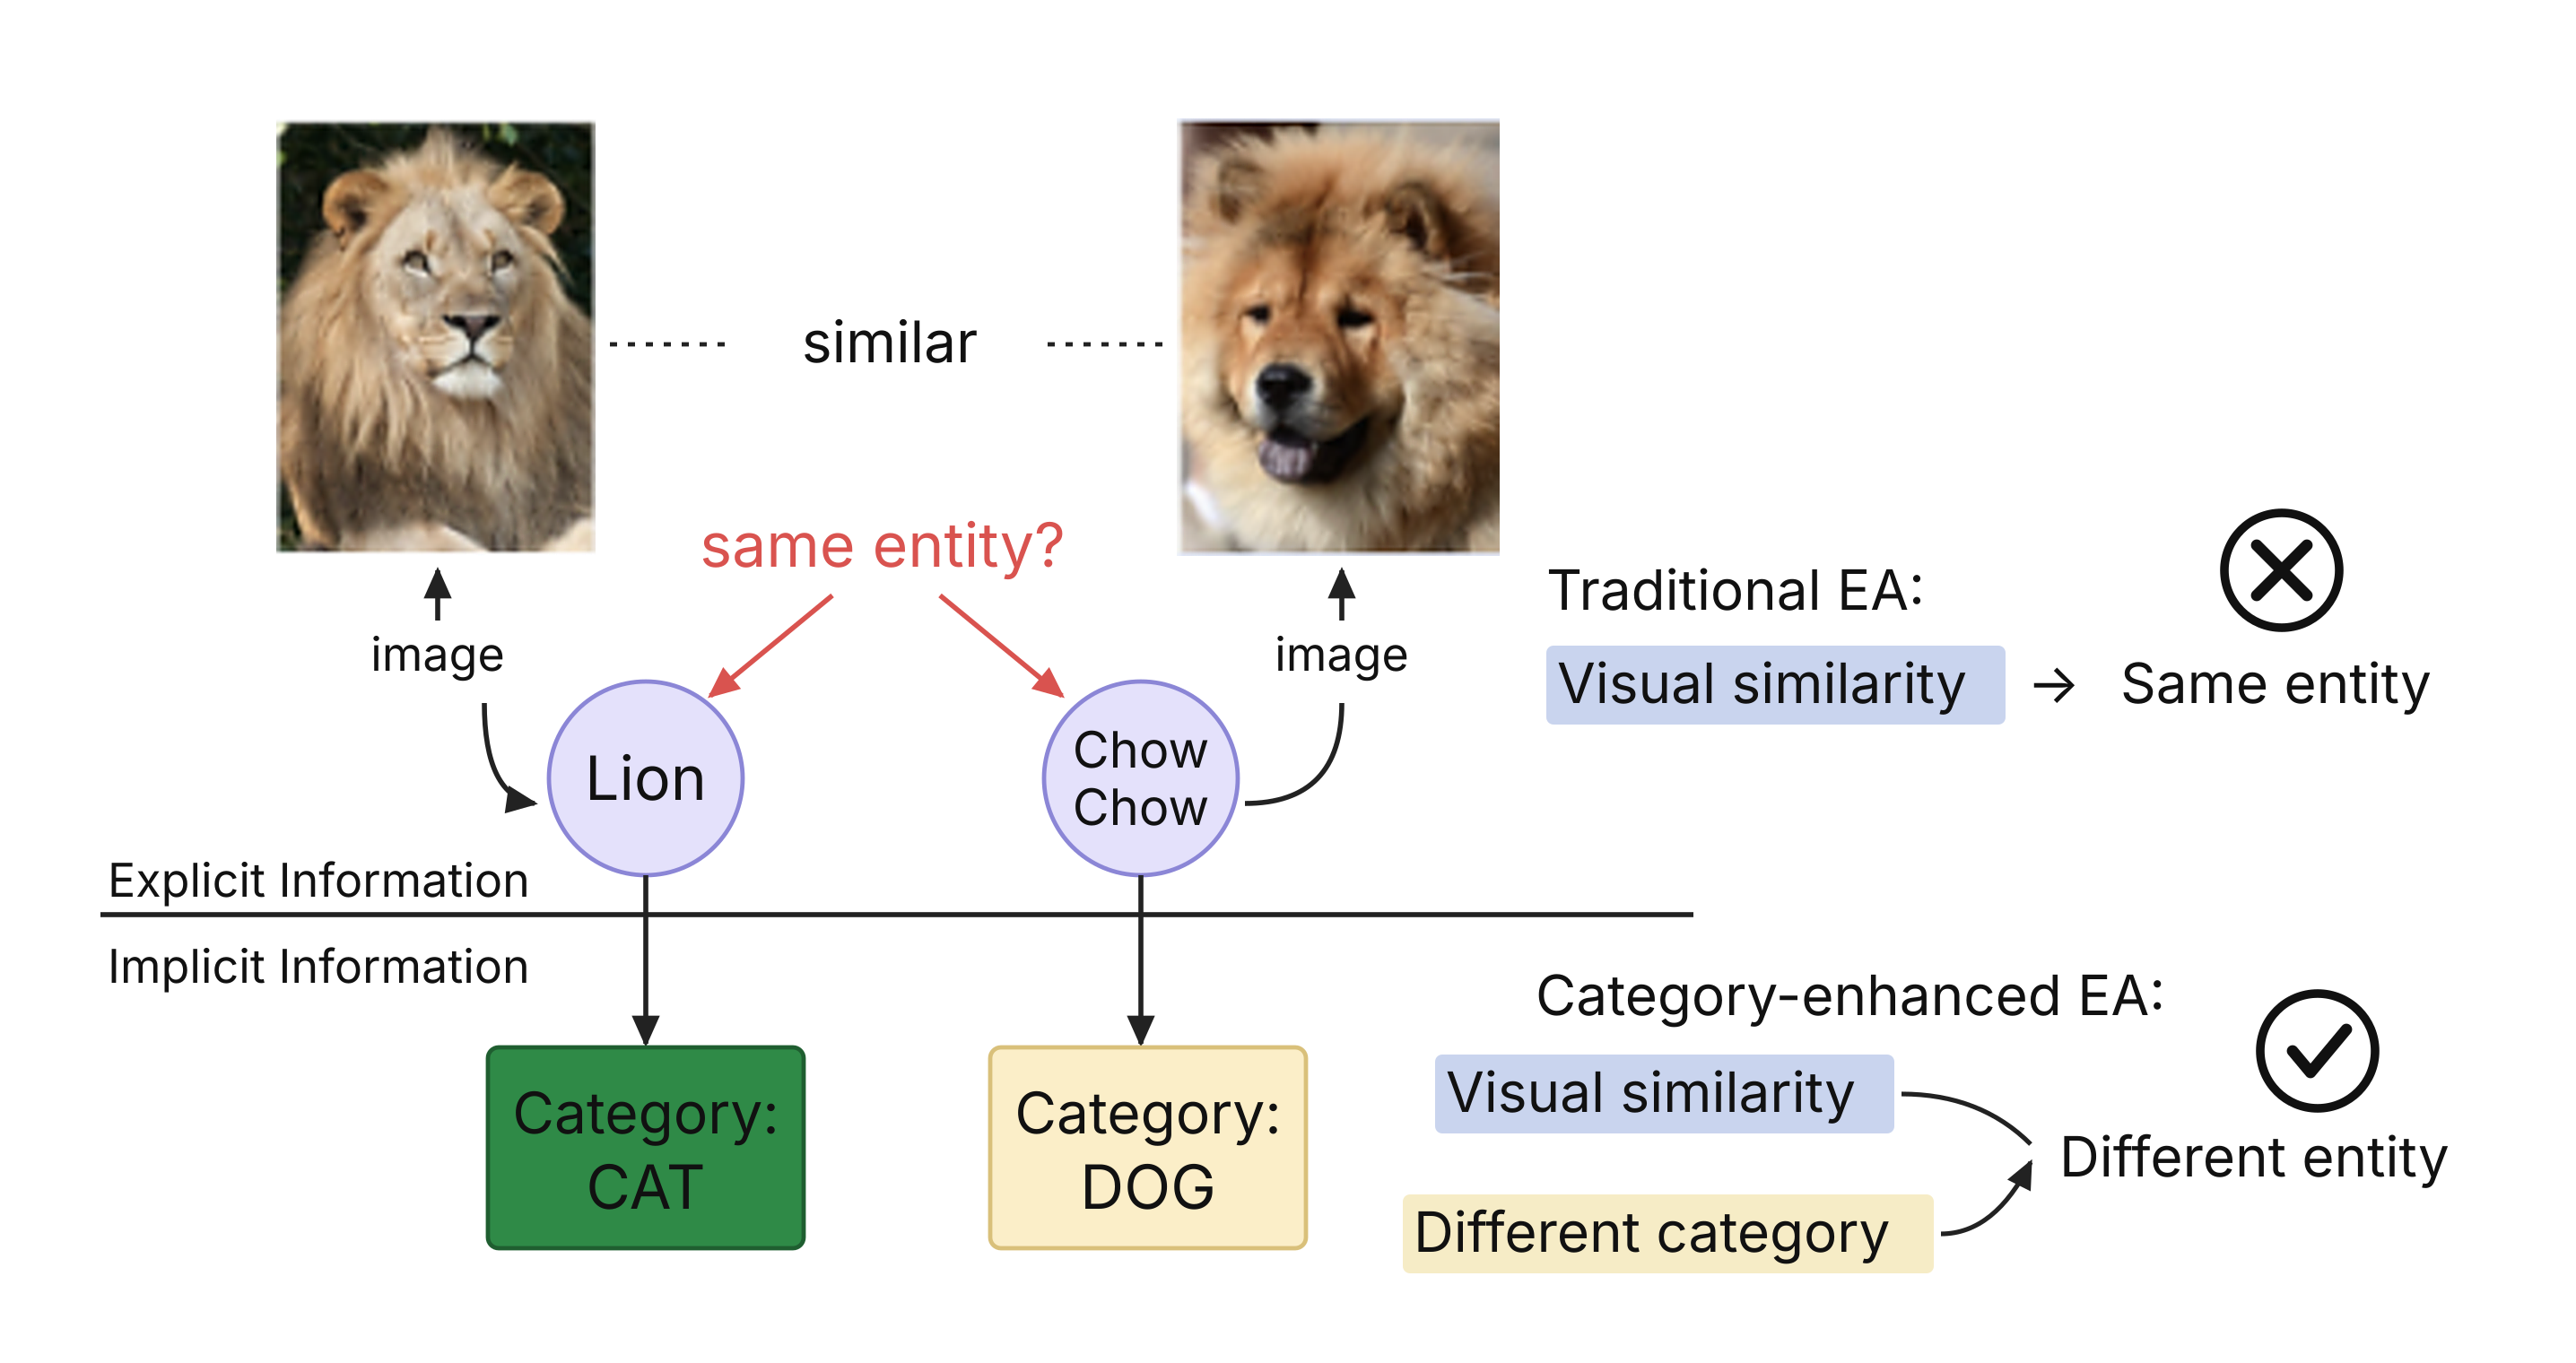
\includegraphics[width=\columnwidth]{figures/exp_1.png}
\caption{Ví dụ về việc căn chỉnh nhầm khi chỉ dựa trên độ tương đồng thị giác, và cách thông tin danh mục ngầm giúp phân biệt. Nguồn: \cite{feng-etal-2025-cateea}.}
\label{fig:cateea_idea}
\end{figure}

Để giải quyết vấn đề này, nhóm tác giả đã đề xuất phương pháp CateEA - với ý tưởng chính là đưa thông tin danh mục ngầm vào quá trình căn chỉnh thực thể để giảm những nhầm lẫn như trên.

\subsection{Phương pháp và phân tích}

CateEA gồm ba modules chính (Hình~\ref{fig:cateea_pipeline}):
\begin{itemize}
    \item \textit{Multi-Modal Encoder (MME):} Mã hoá từng nguồn thông tin rồi tổng hợp thành joint embedding.
    \item \textit{Contrastive Representation Learning (CRL):} Sử dụng phương pháp học tương phản để tinh chỉnh các embedding.
    \item \textit{Category Information Enhancement (CIE):} Khai thác thông tin danh mục ngầm để cải thiện việc căn chỉnh các thực thể.
    
\end{itemize}

\begin{figure*}[t]
\centering
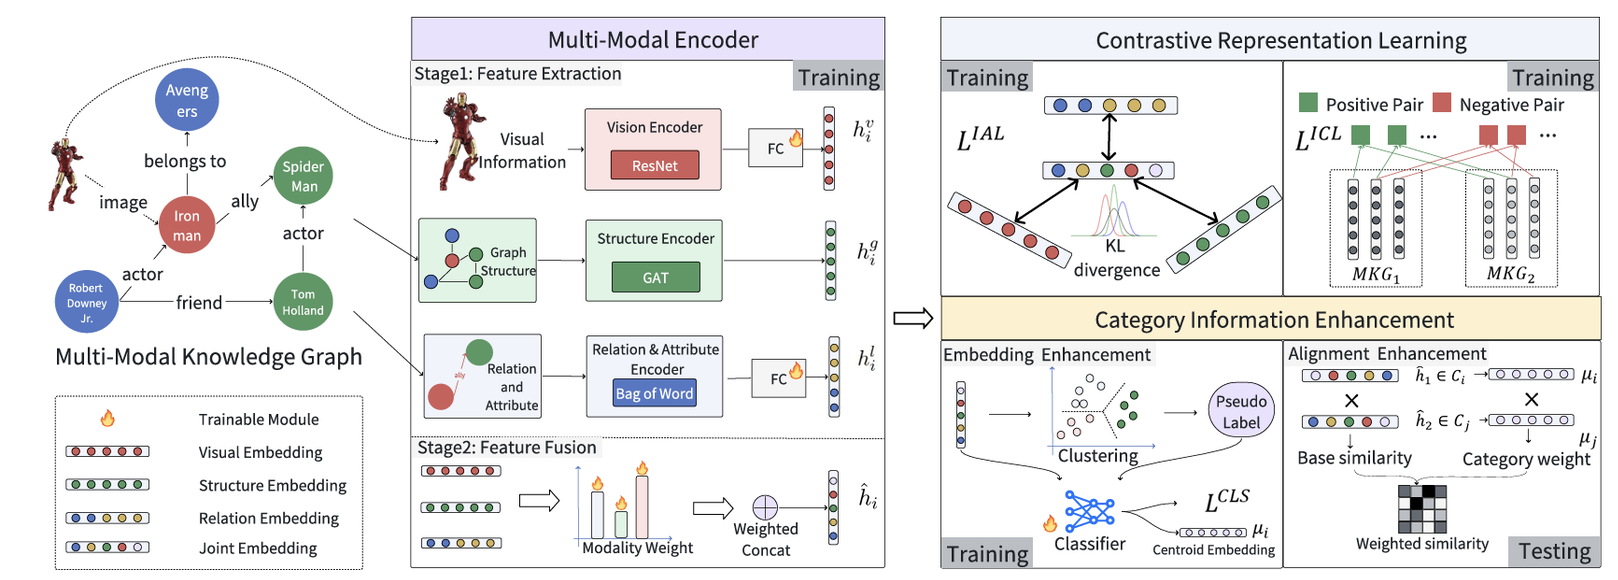
\includegraphics[width=\textwidth]{figures/pipeline.png}
\caption{Kiến trúc tổng quan của CateEA. Các modality được mã hóa rồi kết hợp thành một joint embedding duy nhất. Joint embedding này được tinh chỉnh qua module CRL để các thực thể tương ứng nằm gần nhau hơn. Song song đó, các embedding được phân cụm để tạo pseudo-category, và thông tin danh mục này được dùng để hỗ trợ huấn luyện và điều chỉnh độ tương đồng giữa các cặp thực thể. Nguồn: \cite{feng-etal-2025-cateea}, Fig. 2. Lưu ý: hình gốc chưa đánh dấu GAT là trainable; trong mã nguồn, các tham số GAT vẫn được cập nhật khi huấn luyện.}
\label{fig:cateea_pipeline}
\end{figure*}

\subsubsection{Xây dựng và học biểu diễn đa phương thức} %Hùng
% MME: mã hóa từng nguồn thông tin và kết hợp embedding.
% CRL: vai trò của ICL và IAL.
% Phân tích ý nghĩa và lựa chọn thiết kế ngay tại phần tương ứng.

Hai module MME và CRL là phần nền của CateEA, có nhiệm vụ tạo ra joint embedding của thực thể và học embedding đó cho bài toán căn chỉnh. Hai module này kế thừa nhiều từ các công trình MMEA trước đó như MCLEA\cite{lin-etal-2022-mclea}, MEAformer\cite{chen2023meaformer} nên không phải là đóng góp chính của tác giả. Nhóm chỉ trình bày ở mức cần thiết để hiểu module khai thác danh mục ngầm ở phần sau.

\paragraph{Multi-Modal Encoder (MME)}

MME dùng một bộ encoder riêng cho mỗi phương thức: 
\begin{itemize}
    \item \textit{Với cấu trúc đồ thị:}
        Sử dụng mạng GAT hai tầng để tổng hợp
        thông tin từ các thực thể lân cận thông qua
        cơ chế attention. Mỗi tầng tổng hợp thông tin
        từ các láng giềng trực tiếp, cho phép embedding
        ở tầng cuối tiếp nhận thông tin từ vùng lân cận
        tối đa hai bước (2-hop). Đầu ra là embedding
        cấu trúc $\mathbf{h}^g_i$. %Toàn sửa

    \item \textit{Với quan hệ, thuộc tính và tên}, mỗi loại $l \in \{r, a, n\}$ được biểu diễn bằng bag-of-words rồi đưa qua một lớp tuyến tính $\mathbf{h}^l_i = \mathbf{W}_l \mathbf{u}^l_i + \mathbf{b}_l$. Riêng với tên, vector đầu vào là trung bình các vector GloVe đã huấn luyện sẵn của các từ trong tên.

    \item \textit{Với hình ảnh:} Ảnh của thực thể được đưa qua ResNet-152 đã huấn luyện sẵn, lấy logits của lớp fully connected cuối cùng rồi qua một lớp tuyến tính để được $\mathbf{h}^v_i$.
\end{itemize}

Sau khi có embedding của từng modality, joint embedding được tạo bằng cách nối chúng lại, mỗi modality được nhân với một trọng số attention:
\[
    \hat{\mathbf{h}}_i
    = \bigoplus_{m \in \mathcal{M}}
    \frac{\exp(w_m)}{\sum_{j \in \mathcal{M}} \exp(w_j)}\,\mathbf{h}^m_i.
\]
Ở đây $\mathcal{M}=\{g,r,a,n,v\}$, $\oplus$ là phép nối vector và $w_m$ là trọng số attention học được của modality $m$.


\noindent\textit{Nhận xét của nhóm:} $w_m$ là tham số dùng chung cho mọi thực thể, nên mô hình chỉ học được modality nào nhìn chung đáng tin hơn, chứ không điều chỉnh riêng cho từng thực thể. Cách này đơn giản hơn MEAformer\cite{chen2023meaformer}, nơi trọng số modality thay đổi theo từng thực thể. Khi một thực thể thiếu ảnh hoặc thiếu thuộc tính thì modality đó vẫn được gán trọng số như các thực thể khác. Ngoài ra, nhóm thấy nhóm đặc trưng SF ảnh hưởng rất lớn đến kết quả. Ở cả bài báo và kết quả tái lập trên DBP15K, Hits@1 khi có SF đều trên 94\%, còn khi không có SF chỉ khoảng 74--78\% ở chế độ non-iterative. Điều này cho thấy việc bổ sung nhóm đặc trưng SF cải thiện đáng kể kết quả trên DBP15K. Trong cấu hình tái lập, w/o SF tắt cả đặc trưng tên và ký tự, nên so sánh này chưa tách riêng đóng góp của tên thực thể hay của từng phương thức.

\paragraph{Contrastive Representation Learning (CRL)}

Joint embedding từ MME chưa được đảm bảo là các thực thể tương ứng nằm gần nhau, nên CRL huấn luyện embedding theo hướng đó. Với mỗi cặp thực thể $(e^1_i, e^2_i)$ trong tập seed, các thực thể còn lại của cả hai đồ thị được xem là mẫu âm $\mathcal{N}^{neg}_i$. Xác suất căn chỉnh của modality $m$ được tính như sau:
\[
    q_m(e^1_i, e^2_i)
    = \frac{\delta_m(e^1_i, e^2_i)}
    {\delta_m(e^1_i, e^2_i)
    + \sum_{e_j \in \mathcal{N}^{neg}_i}
    \left[\delta_m(e_j, e^1_i) + \delta_m(e^2_i, e_j)\right]},
\]
với $\delta_m(u,v) = \exp\!\left(f_m(u)^\top f_m(v) / \tau_1\right)$, $f_m(\cdot)$ là encoder của modality $m$ và $\tau_1$ là nhiệt độ.

Module CRL gồm hai hàm loss:
\begin{itemize}
    \item \textit{ICL (Intra-modal Contrastive Learning):} Với từng modality, kéo cặp thực thể tương ứng lại gần nhau và đẩy các thực thể khác ra xa:
    \[
        \mathcal{L}^{ICL}_m = -\mathbb{E}_{i \in B}\log
        \tfrac{1}{2}\left[q_m(e^1_i, e^2_i) + q_m(e^2_i, e^1_i)\right].
    \]
  \item \textit{IAL (Inter-modal Alignment Learning):} Tính các vector phân phối xác suất $\mathbf{q}'_o$ từ joint embedding và $\mathbf{q}'_m$ từ modality $m$ trên cùng tập ứng viên, sử dụng nhiệt độ $\tau_2$. Sau đó, sử dụng KL divergence để đưa phân phối của modality $m$ tiệm cận với phân phối của joint embedding theo cả hai chiều:

    \begin{equation}
        \begin{aligned}
        \mathcal{L}^{IAL}_m
        = \frac{1}{2}\mathbb{E}_{i \in B}\Big[
        &\operatorname{KL}\big(
        \mathbf{q}'_o(e^1_i,\cdot)
        \,\|\, \mathbf{q}'_m(e^1_i,\cdot)
        \big)\\
        +&\operatorname{KL}\big(
        \mathbf{q}'_o(e^2_i,\cdot)
        \,\|\, \mathbf{q}'_m(e^2_i,\cdot)
        \big)
        \Big].
        \end{aligned}
    \end{equation}
    Ở đây $\mathbf{q}'_m(u,\cdot)$ là vector xác suất của các
    ứng viên khi truy vấn là $u$; mỗi phần tử tương ứng với một
    ứng viên. KL được tính trên toàn bộ hai vector phân phối,
    không chỉ trên xác suất của riêng cặp thực thể tương ứng.

\end{itemize}

Nhóm hiểu hai hàm loss này bổ sung cho nhau. ICL chỉ xét từng modality riêng lẻ nên các modality có thể học theo những hướng khác nhau, còn IAL buộc từng modality phải nhất quán với joint embedding. Nhờ vậy một modality yếu hoặc nhiễu (chẳng hạn ảnh không rõ) vẫn nhận được tín hiệu từ các modality mạnh hơn.

\subsubsection{Khai thác thông tin danh mục ngầm}
% CEE: phân cụm, tạo nhãn giả và học phân loại.
% CAE: tính trọng số danh mục và điều chỉnh điểm căn chỉnh.
% Phân biệt huấn luyện với suy luận; phân tích các giả định.

Đây là module mang tính novelty và là đóng góp chính của CateEA.

Module này có hai thành phần là \textit{Category Embedding Enhancement} và \textit{Category Alignment Enhancement}:

\paragraph{Category Embedding Enhancement (CEE)}


Đầu tiên, mô hình đã có joint embedding của thực thể, được tạo bởi module MME và được tối ưu thông qua CRL. Nhiệm vụ của CEE là phân cụm những embedding này bằng K-Medoids và lấy kết quả phân cụm làm nhãn danh mục giả (pseudo-category label). Sau đó, classifier học dự đoán nhãn giả từ embedding. Loss phân loại cross-entropy được kết hợp với loss căn chỉnh và truyền ngược về encoder để điều chỉnh biểu diễn. Tác giả nói rằng cơ chế này tương tự ý tưởng trong công trình DeepCluster năm 2018 \cite{caron2018deepcluster}.

Loss phân loại không trực tiếp kéo các embedding cùng cụm lại gần nhau, mà khuyến khích encoder tạo ra các embedding có những đặc điểm giúp phân biệt các danh mục với nhau. Luồng gradient từ loss phân loại về encoder được xác nhận trong code; tuy nhiên, việc ghép nhãn giả với embedding có sai khác sẽ được phân tích ở phần đối chiếu mã nguồn.

Việc phân cụm này không tự tạo thêm dữ liệu hay tri thức từ bên ngoài. Nó tổ chức lại những đặc điểm đã có trong không gian embedding, rồi biến cách tổ chức đó thành tín hiệu giám sát bổ sung. Ngoài ra "danh mục ngầm - implicit category" chưa chắc đã tương ứng với các danh mục thực sự ngoài thế giới thật. Phương pháp của tác giả đề xuất cơ chế này dựa trên ý tưởng khai thác thông tin danh mục ngầm ngoài thế giới thực, nhưng tác giả chưa chỉ ra các embedding trong cùng một cụm có thuộc một danh mục nào đó ngoài thực tế hay không.


Ngoài loss của classifier, nhóm còn quan tâm đến cấu trúc phân cụm. Paper sử dụng K-Medoids để chia các embedding thành $k$ cụm ở một cấp, với $k$ được xác định trước, không xây dựng các cụm cha-con hay phân cụm lồng nhau. Tác giả giải thích việc chọn K-Medoids dựa trên đặc điểm sử dụng điểm dữ liệu thực làm đại diện cụm và khả năng chống chịu nhiễu, outlier,... Tuy nhiên, paper chưa cung cấp thực nghiệm so sánh với các phương pháp phân cụm khác để kiểm chứng lợi ích của lựa chọn này trong CateEA. Phần phân tích tham số của tác giả chỉ khảo sát ảnh hưởng của số cụm $k$ khi sử dụng K-Medoids \cite{feng-etal-2025-cateea}. Và lưu ý rằng việc phân cụm chỉ xảy ra ở quá trình training. Ở quá trình inference, encoder MME đã được huấn luyện với các mục tiêu CRL tạo ra embedding để classifier dự đoán nhãn danh mục ngầm, không chạy lại CRL hay thuật toán clustering.

\paragraph{Category Alignment Enhancement (CAE)}

Thành phần CEE đã tác động vào embedding trong quá trình training, còn CAE tiếp tục sử dụng thông tin danh mục để điều chỉnh xếp hạng ứng viên. Trong mã nguồn, ở giai đoạn suy luận, classifier dự đoán nhãn danh mục giả $c_x$, $c_y$ cho hai thực thể $x$, $y$ tương ứng từ joint embedding mà không chạy lại K-Medoids. Các thực thể cùng nhãn trong mỗi đồ thị được gom nhóm thành $C_i$. Bốn bước CAE được mô tả ở paper:

\begin{itemize}
    \item Tính centroid của mỗi danh mục bằng trung bình joint embedding của các thực thể thuộc danh mục đó.
    \[
        \boldsymbol{\mu}_i
        = \frac{1}{|C_i|}
        \sum_{x \in C_i} \hat{\mathbf{h}}_x.
    \]
    \item Đo khoảng cách giữa hai danh mục, rồi chuyển thành độ tương đồng. Centroid càng gần nhau thì $s_{ij}$ càng lớn.

    \[
        d_{ij} = \|\boldsymbol{\mu}_i - \boldsymbol{\mu}_j\|_2,
        \qquad
        s_{ij} = \frac{1}{1 + d_{ij}}.
    \]
    \item Chuẩn hóa trọng số bằng softmax:

    \[
        w_{ij}
        = \frac{\exp(s_{ij})}
        {\sum_{k=1}^{C} \exp(s_{ik})}.
    \]
    \item Điều chỉnh độ tương đồng thực thể:
    \[
        S'(x,y)
        = w_{c_x,c_y}\,S(x,y).
    \]
\end{itemize}

Ký hiệu $\hat{\mathbf{h}}_x$ là joint embedding của $x$; $\boldsymbol{\mu}_i$ là centroid của $C_i$; $C$ là số danh mục. $d_{ij},s_{ij},w_{ij}$ lần lượt là khoảng cách, độ tương đồng và trọng số giữa hai danh mục. $S,S'$ là độ tương đồng thực thể trước và sau điều chỉnh.

\noindent\textit{Một nhận xét của nhóm:} Paper chọn K-Medoids vì paper lý giải rằng medoid là điểm dữ liệu thực, giúp tâm cụm mang tính đại diện và ít ảnh hưởng bởi nhiễu; nhưng ở giai đoạn suy luận lại dùng centroid (vector trung bình) không nhất thiết trùng với embedding của bất kì thực thể nào để tính khoảng cách giữa các danh mục. Paper không phân tích rõ lý do lựa chọn centroid ở bước này.

Nhóm cũng cho rằng CAE đang dựa trên giả thuyết: khoảng cách giữa các centroid thể hiện mức độ phù hợp giữa các danh mục cho việc căn chỉnh. Vấn đề nhóm thấy là centroid là biểu diễn giá trị trung bình, chưa phản ánh độ phân tán thực thể bên trong nhóm đó. Ngoài ra nếu classifier dự đoán sai nhãn, sai số này có thể ảnh hưởng đến cả centroid và trọng số hiệu chỉnh. Vì vậy, CAE không đảm bảo luôn cải thiện xếp hạng. 

Hình~\ref{alg:cateea} tóm tắt luồng khai thác danh mục ngầm
được nhóm diễn giải lại theo mô tả phương pháp trong bài báo.
Giả mã tách hai giai đoạn huấn luyện và suy luận; các sai khác
của mã nguồn công khai được phân tích tại
mục~\ref{sec:cateea_code_comparison}.

\begin{figure}[t]
\footnotesize
\begin{algorithmic}[1]
\REQUIRE Graphs $G_1,G_2$ with entity sets $E_1,E_2$;
    training alignment pairs $\mathcal{A}$; number of clusters $C$.
\ENSURE Ranked candidates for each query entity.
\STATE Initialize encoder $f_\theta$ and classifier $g_\phi$.
\STATE \textbf{Training: clustering and pseudo-label learning}
\REPEAT
    \STATE Compute $\hat{\mathbf{h}}_e=f_\theta(e)$ for
        $e\in E_1\cup E_2$.
    \STATE Cluster all embeddings with K-Medoids;
        use cluster indices as pseudo-labels $y_e$.
    \FOR{each batch of alignment pairs from $\mathcal{A}$}
        \STATE Recompute embeddings for entities in the batch.
        \STATE Predict category distributions
            $\mathbf{p}_e=g_\phi(\hat{\mathbf{h}}_e)$.
        \STATE Compute $\mathcal{L}_{\mathrm{cls}}$
            as cross-entropy between $\mathbf{p}_e$ and $y_e$.
        \STATE $\mathcal{L}=\mathcal{L}_{\mathrm{align}}
            +\lambda\mathcal{L}_{\mathrm{cls}}$.
        \STATE Backpropagate to update $\theta,\phi$;
            keep pseudo-labels fixed during this update.
    \ENDFOR
\UNTIL{the training stopping criterion is met}
\STATE \textbf{Inference: classification and ranking adjustment}
\STATE Recompute embeddings using the trained encoder.
\FOR{$g\in\{1,2\}$}
    \STATE Predict $c_e=\arg\max_c g_\phi(
        \hat{\mathbf{h}}_e)_c$ for each $e\in E_g$.
    \STATE Form groups $C_a^{(g)}=\{e\in E_g:c_e=a\}$;
        compute each centroid $\boldsymbol{\mu}_a^{(g)}$
        as the mean embedding of its group.
\ENDFOR
\STATE For each cross-graph category pair, compute
    $d_{ab}=\|\boldsymbol{\mu}_a^{(1)}
    -\boldsymbol{\mu}_b^{(2)}\|_2$ and $s_{ab}=1/(1+d_{ab})$.
\STATE Normalize $w_{ab}=\exp(s_{ab})/\sum_k\exp(s_{ak})$.
\FOR{each query entity $x\in E_1$}
    \STATE For each candidate $y\in E_2$, compute
        $S'(x,y)=w_{c_x,c_y}S(x,y)$.
    \STATE Rank candidates by decreasing $S'(x,y)$;
        apply the same procedure in the reverse direction.
\ENDFOR
\end{algorithmic}
\caption{Luồng khai thác danh mục ngầm do nhóm diễn giải lại
    theo mô tả CateEA~\cite{feng-etal-2025-cateea}.
    Lược đồ huấn luyện minh họa việc tạo nhãn giả rồi học với
    các nhãn đó, không đặc tả lịch cập nhật của mã nguồn.
    K-Medoids chỉ dùng trong huấn luyện; suy luận dùng classifier.
    Các centroid được tính cho những nhóm không rỗng.}
\label{alg:cateea}
\end{figure}
\subsection{Tái lập thực nghiệm}

% Declare wide result tables early to keep them within the CateEA section.
\begin{table*}[!t]
\centering
\caption{So sánh Hits@1, Hits@10 và MRR (\%) trên DBP15K; đối chiếu Tables 1--2 của bài báo.}
\label{tab:cateea_dbp15k}
\small
\renewcommand{\arraystretch}{1.12}
\setlength{\tabcolsep}{4pt}
\begin{tabular}{@{}llrrr@{\hspace{10pt}}rrr@{\hspace{10pt}}rrr@{}}
\toprule
\textbf{Cấu hình} & \textbf{Kết quả} & \multicolumn{3}{c}{\textbf{ZH-EN}} & \multicolumn{3}{c}{\textbf{JA-EN}} & \multicolumn{3}{c}{\textbf{FR-EN}} \\
\cmidrule(lr){3-5}\cmidrule(lr){6-8}\cmidrule(lr){9-11}
 &  & \textbf{H@1$\uparrow$} & \textbf{H@10$\uparrow$} & \textbf{MRR$\uparrow$} & \textbf{H@1$\uparrow$} & \textbf{H@10$\uparrow$} & \textbf{MRR$\uparrow$} & \textbf{H@1$\uparrow$} & \textbf{H@10$\uparrow$} & \textbf{MRR$\uparrow$} \\
\midrule
Non-iter w/o SF & Paper & 77.60 & 95.50 & 83.90 & 77.20 & 96.30 & 84.00 & 78.60 & 97.20 & 85.50 \\
 & Tái lập & \cateearun{smwb7h2s}{73.75} & \cateearun{smwb7h2s}{94.82} & \cateearun{smwb7h2s}{81.27} & \cateearun{1i8acfog}{76.02} & \cateearun{1i8acfog}{96.19} & \cateearun{1i8acfog}{83.34} & \cateearun{cs880n51}{78.14} & \cateearun{cs880n51}{97.25} & \cateearun{cs880n51}{85.22} \\
 & $\Delta$ & \deltaneg{-3.85} & \deltaneg{-0.68} & \deltaneg{-2.63} & \deltaneg{-1.18} & \deltaneg{-0.11} & \deltaneg{-0.66} & \deltaneg{-0.46} & \deltapos{+0.05} & \deltaneg{-0.28} \\
\addlinespace[3pt]
Non-iter w/ SF & Paper & 94.50 & 99.30 & 96.40 & 97.20 & 99.80 & 98.70 & 99.10 & 100.00 & 99.50 \\
 & Tái lập & \cateearun{ouxqphvg}{94.20} & \cateearun{ouxqphvg}{99.27} & \cateearun{ouxqphvg}{96.13} & \cateearun{i448247f}{97.13} & \cateearun{i448247f}{99.85} & \cateearun{i448247f}{98.25} & \cateearun{h9llx682}{99.01} & \cateearun{h9llx682}{99.98} & \cateearun{h9llx682}{99.43} \\
 & $\Delta$ & \deltaneg{-0.30} & \deltaneg{-0.03} & \deltaneg{-0.27} & \deltaneg{-0.07} & \deltapos{+0.05} & \deltaneg{-0.45} & \deltaneg{-0.09} & \deltaneg{-0.02} & \deltaneg{-0.07} \\
\addlinespace[3pt]
Iter w/o SF & Paper & 83.90 & 97.10 & 88.70 & 85.10 & 97.80 & 89.90 & 86.20 & 98.50 & 90.80 \\
 & Tái lập & \cateearun{yhxmaaiy}{79.58} & \cateearun{yhxmaaiy}{95.69} & \cateearun{yhxmaaiy}{85.48} & \cateearun{anh3017u}{82.68} & \cateearun{anh3017u}{97.07} & \cateearun{anh3017u}{88.11} & \cateearun{yfsixay2}{84.77} & \cateearun{yfsixay2}{98.00} & \cateearun{yfsixay2}{89.78} \\
 & $\Delta$ & \deltaneg{-4.32} & \deltaneg{-1.41} & \deltaneg{-3.22} & \deltaneg{-2.42} & \deltaneg{-0.73} & \deltaneg{-1.79} & \deltaneg{-1.43} & \deltaneg{-0.50} & \deltaneg{-1.02} \\
\addlinespace[3pt]
Iter w/ SF & Paper & 97.40 & 99.80 & 98.40 & 99.20 & 99.90 & 99.30 & 99.70 & 100.00 & 99.80 \\
 & Tái lập & \cateearun{vzdpd3hi}{97.24} & \cateearun{vzdpd3hi}{99.71} & \cateearun{vzdpd3hi}{98.22} & \cateearun{0sp0eyep}{98.84} & \cateearun{0sp0eyep}{99.97} & \cateearun{0sp0eyep}{99.31} & \cateearun{xvueasz7}{99.64} & \cateearun{xvueasz7}{100.00} & \cateearun{xvueasz7}{99.81} \\
 & $\Delta$ & \deltaneg{-0.16} & \deltaneg{-0.09} & \deltaneg{-0.18} & \deltaneg{-0.36} & \deltapos{+0.07} & \deltapos{+0.01} & \deltaneg{-0.06} & 0.00 & \deltapos{+0.01} \\
\bottomrule
\end{tabular}
\vspace{3pt}
\begin{tablenotes}[flushleft]
\footnotesize
\item \textit{Nhấn vào các số liệu có nền xám
để xem kết quả thực nghiệm tương ứng trên W\&B.}
\end{tablenotes}
\end{table*}

\begin{table*}[!t]
\centering
\caption{So sánh Hits@1, Hits@10 và MRR (\%) trên MMKB; đối chiếu Tables 3--4 của bài báo.}
\label{tab:cateea_mmkb}
\small
\renewcommand{\arraystretch}{1.12}
\setlength{\tabcolsep}{6pt}
\begin{tabular}{@{}lllrrr@{\hspace{14pt}}rrr@{}}
\toprule
\textbf{Chế độ} & \textbf{Tỷ lệ} & \textbf{Kết quả} & \multicolumn{3}{c}{\textbf{FB15K-DB15K}} & \multicolumn{3}{c}{\textbf{FB15K-YAGO15K}} \\
\cmidrule(lr){4-6}\cmidrule(lr){7-9}
 &  &  & \textbf{H@1$\uparrow$} & \textbf{H@10$\uparrow$} & \textbf{MRR$\uparrow$} & \textbf{H@1$\uparrow$} & \textbf{H@10$\uparrow$} & \textbf{MRR$\uparrow$} \\
\midrule
Non-iter & 20\% & Paper & 49.30 & 75.90 & 58.40 & 40.20 & 67.50 & 49.70 \\
 &  & Tái lập & \cateearun{dccl235x}{48.88} & \cateearun{dccl235x}{75.65} & \cateearun{dccl235x}{58.18} & \cateearun{u7l7rzah}{38.84} & \cateearun{u7l7rzah}{66.26} & \cateearun{u7l7rzah}{48.22} \\
 &  & $\Delta$ & \deltaneg{-0.42} & \deltaneg{-0.25} & \deltaneg{-0.22} & \deltaneg{-1.36} & \deltaneg{-1.24} & \deltaneg{-1.48} \\
\addlinespace[3pt]
Non-iter & 50\% & Paper & 67.40 & 87.40 & 74.50 & 60.80 & 82.90 & 68.60 \\
 &  & Tái lập & \cateearun{vckjpp3o}{66.01} & \cateearun{vckjpp3o}{86.16} & \cateearun{vckjpp3o}{73.20} & \cateearun{9060trns}{60.19} & \cateearun{9060trns}{81.83} & \cateearun{9060trns}{67.84} \\
 &  & $\Delta$ & \deltaneg{-1.39} & \deltaneg{-1.24} & \deltaneg{-1.30} & \deltaneg{-0.61} & \deltaneg{-1.07} & \deltaneg{-0.76} \\
\addlinespace[3pt]
Non-iter & 80\% & Paper & 79.90 & 93.30 & 84.90 & 74.20 & 91.20 & 80.50 \\
 &  & Tái lập & \cateearun{92xpyrkt}{77.16} & \cateearun{92xpyrkt}{91.61} & \cateearun{92xpyrkt}{82.52} & \cateearun{iovu8zta}{74.22} & \cateearun{iovu8zta}{90.82} & \cateearun{iovu8zta}{80.36} \\
 &  & $\Delta$ & \deltaneg{-2.74} & \deltaneg{-1.69} & \deltaneg{-2.38} & \deltapos{+0.02} & \deltaneg{-0.38} & \deltaneg{-0.14} \\
\addlinespace[3pt]
Iter & 20\% & Paper & 59.90 & 82.20 & 67.50 & 51.80 & 74.50 & 59.40 \\
 &  & Tái lập & \cateearun{gustc0d9}{62.31} & \cateearun{gustc0d9}{82.45} & \cateearun{gustc0d9}{69.39} & \cateearun{ownvumgr}{52.17} & \cateearun{ownvumgr}{73.46} & \cateearun{ownvumgr}{59.58} \\
 &  & $\Delta$ & \deltapos{+2.41} & \deltapos{+0.25} & \deltapos{+1.89} & \deltapos{+0.37} & \deltaneg{-1.04} & \deltapos{+0.18} \\
\addlinespace[3pt]
Iter & 50\% & Paper & 70.50 & 88.20 & 76.40 & 64.00 & 84.40 & 70.80 \\
 &  & Tái lập & \cateearun{mdwrjgz5}{70.55} & \cateearun{mdwrjgz5}{86.93} & \cateearun{mdwrjgz5}{76.35} & \cateearun{wywowfuy}{64.43} & \cateearun{wywowfuy}{82.53} & \cateearun{wywowfuy}{70.81} \\
 &  & $\Delta$ & \deltapos{+0.05} & \deltaneg{-1.27} & \deltaneg{-0.05} & \deltapos{+0.43} & \deltaneg{-1.87} & \deltapos{+0.01} \\
\addlinespace[3pt]
Iter & 80\% & Paper & 80.60 & 93.40 & 85.30 & 74.60 & 91.50 & 80.70 \\
 &  & Tái lập & \cateearun{t0eainhm}{80.18} & \cateearun{t0eainhm}{92.55} & \cateearun{t0eainhm}{84.65} & \cateearun{oxqvbkz1}{74.71} & \cateearun{oxqvbkz1}{89.33} & \cateearun{oxqvbkz1}{79.98} \\
 &  & $\Delta$ & \deltaneg{-0.42} & \deltaneg{-0.85} & \deltaneg{-0.65} & \deltapos{+0.11} & \deltaneg{-2.17} & \deltaneg{-0.72} \\
\bottomrule
\end{tabular}
\end{table*}


\subsubsection{Thiết lập thực nghiệm}

Nhóm sử dụng mã nguồn công khai của tác giả và bổ sung các script chạy, ghi nhận kết quả bằng Weights \& Biases (W\&B), cùng chức năng lưu checkpoint. Mã nguồn và hướng dẫn chạy lại được cung cấp tại \href{https://github.com/keiranoluv/Reproduce_CateEA}{GitHub}.

Theo cấu hình được ghi nhận trong repository, môi trường thực nghiệm sử dụng Ubuntu 24.04, GPU NVIDIA GeForce RTX 5090 với 32 GB VRAM, Python 3.12 và PyTorch 2.13.0 với CUDA 13.0. Dữ liệu được lấy từ gói dữ liệu do MEAformer cung cấp, gồm:
\begin{itemize}
    \item \textit{DBP15K:} ba cặp ngôn ngữ ZH-EN, JA-EN và FR-EN, với tỷ lệ cặp thực thể huấn luyện là 30\%.
    \item \textit{MMKB:} FB15K-DB15K và FB15K-YAGO15K, với các tỷ lệ huấn luyện 20\%, 50\% và 80\%.
\end{itemize}

Trên DBP15K, nhóm chạy hai chế độ non-iterative và iterative, mỗi chế độ có cấu hình sử dụng và không sử dụng surface form (SF). Trong mã nguồn, cấu hình w/o SF tắt cả đặc trưng tên và ký tự. Trên MMKB, nhóm chạy hai chế độ với ba tỷ lệ huấn luyện, không sử dụng các đặc trưng này. Tổng cộng có 24 cấu hình thực nghiệm.

Các script đặt số epoch là 1000, learning rate $5\times10^{-4}$, batch size 512, random seed 42, $\tau_1=0.1$, $\tau_2=0.4$ và CSLS với $k=3$. Mô hình được đánh giá sau mỗi 50 epoch. Với chế độ iterative, quá trình bổ sung cặp thực thể được bật từ epoch có chỉ số 500. Chi tiết từng cấu hình được lưu trong các script của repository.

Mã nguồn ghi nhận Hits@1, Hits@10, Hits@50 và MRR theo hai chiều căn chỉnh. Checkpoint tốt nhất được chọn theo Hits@1 trung bình hai chiều của nhánh đánh giá thông thường (\texttt{test}). Nhánh có điều chỉnh danh mục (\texttt{weighted}) được đánh giá và ghi nhận riêng tại cùng checkpoint. Nhóm sử dụng kết quả của nhánh \texttt{weighted} tại checkpoint này để so sánh với bài báo.


\noindent\textit{Giới hạn của giao thức đánh giá:} Nhóm \textbf{chọn checkpoint dựa trên Hits@1 của tập kiểm tra}, thay vì một tập validation độc lập. Vì vậy, tập kiểm tra đồng thời tham gia lựa chọn mô hình và đánh giá kết quả cuối cùng, có thể khiến kết quả được báo cáo lạc quan hơn so với đánh giá trên dữ liệu chưa tham gia lựa chọn. Các kết quả CateEA cần được diễn giải cùng giới hạn này.


Các lần chạy được theo dõi tại \href{https://forge.coreweave.com/wandb/keiranoluv-hcmus/cateea-reproduction}{W\&B}.
% Bổ sung link run/report tương ứng ngay tại từng bảng kết quả.


\subsubsection{Kết quả và phân tích}

Bảng~\ref{tab:cateea_dbp15k} và Bảng~\ref{tab:cateea_mmkb}
so sánh Hits@1, Hits@10 và MRR (\%) giữa bài báo và kết quả tái lập.
$\Delta$ là chênh lệch giữa kết quả tái lập và bài báo,
tính theo \%. Bấm vào số liệu tái lập sẽ dẫn
đến run W\&B tương ứng.





Trên DBP15K (Bảng~\ref{tab:cateea_dbp15k}), Hits@1 tái lập
thấp hơn bài báo ở toàn bộ cấu hình. Khi sử dụng SF,
chênh lệch nhỏ hơn 0.4\%. Khi không sử dụng SF,
chênh lệch rõ hơn, lớn nhất là 4.32\% ở
ZH-EN iterative. Nhóm tái hiện được xu hướng các cấu hình
có SF đạt kết quả cao hơn và iterative cải thiện so với
non-iterative ở các thiết lập tương ứng. Tuy nhiên, các
kết quả này chưa đủ xác định nguyên nhân của chênh lệch
với bài báo.





Trên MMKB (Bảng~\ref{tab:cateea_mmkb}), Hits@1 tái lập
non-iterative thấp hơn bài báo ở phần lớn cấu hình.
Với iterative, năm trong sáu cấu hình đạt kết quả cao hơn
bài báo trong lần chạy này, đáng chú ý nhất là
FB15K-DB15K với tỷ lệ 20\%, cao hơn 2.41\%.

Ở các cấu hình MMKB iterative, Hits@10 chỉ cao hơn bài báo
trong một cấu hình, còn MRR cao hơn trong ba cấu hình.
Xu hướng chênh lệch với bài báo không đồng nhất giữa các metric.

Trong các kết quả tái lập, iterative đều cải thiện so với
non-iterative ở cùng bộ dữ liệu và tỷ lệ huấn luyện.
Kết quả cũng tăng khi tỷ lệ cặp huấn luyện tăng.
Tuy nhiên, vì mỗi cấu hình sử dụng một random seed,
nhóm chưa đánh giá được độ biến thiên giữa các lần chạy;
những chênh lệch nhỏ chưa đủ chứng minh sự cải thiện ổn định.

\subsection{Đánh giá và thảo luận}

\subsubsection{Đối chiếu bài báo với mã nguồn}
\label{sec:cateea_code_comparison}

Trong quá trình tìm hiểu và tái lập, nhóm ghi nhận một số sai khác giữa mô tả phương pháp và mã nguồn công khai. 

% \begin{itemize}
%     \item 
%     Paper viết việc phân cụm dựa trên joint embedding của một thực thể. Trong code, với mỗi cặp thực thể tương ứng đã biết, hai embedding này được cộng lại thành một vector mới rồi được đưa vào phân cụm.

%     \item 
%     Sau khi tạo nhãn giả cho từng cặp thực thể ở bước trên, code ghép các nhãn này với thực thể theo thứ tự trong danh sách ban đầu, thay vì gán nhãn cho đúng hai thực thể thuộc cặp tương ứng.
%     \item 
%     Paper nói rằng số cụm $C=10$ nhưng tác giả lại hardcode là $C=5$.

%     \item 
%     Paper đưa các độ tương đồng danh mục qua softmax để chuẩn hoá còn code lại thực hiện phép chia một phần tử cho tổng.

%     \item 
%     Trong paper, "trọng số danh mục" được nhân với "độ tương đồng thực thể", điểm càng lớn thì ứng viên càng được ưu tiên. Tuy nhiên, code lại nhân "trọng số danh mục" với "khoảng cách thực thể". "Trọng số danh mục" là đại lượng càng lớn càng tốt, "khoảng cách thực thể" là một đại lượng càng nhỏ càng tốt nếu ta muốn xét đến độ tương đồng, vậy mà code lại nhân hai đại lượng này với nhau.
% \end{itemize}

Nhóm đối chiếu mã nguồn CateEA tại commit
\texttt{8c277f3} với mô tả phương pháp trong bài báo và ghi nhận:
\begin{itemize}
  \item \textit{Đầu vào phân cụm:} mã nguồn tạo một vector cho
  mỗi cặp căn chỉnh $(u_i,v_i)$ bằng phép cộng
  $\hat{h}_{u_i}+\hat{h}_{v_i}$, rồi phân cụm các vector này,
  thay vì trực tiếp phân cụm từng biểu diễn thực thể.
  \footnote{\href{https://github.com/Melkor0007/CateEA/blob/8c277f3292b98f22aaaecb75d01ac44487cefed6/src/myrun.py\#L461-L474}{CateEA: tạo đầu vào và nhãn phân cụm.}}

  \item \textit{Ghép nhãn giả:} nhãn được tạo theo thứ tự các
  cặp trong \texttt{train\_ill}, nhưng loss phân loại sử dụng
  \texttt{joint\_emb[si:end\_idx]} cùng
  \texttt{cluster\_labels[si:end\_idx]}, không truy xuất
  embedding theo ID của hai thực thể trong cặp tương ứng.
  \footnote{\href{https://github.com/Melkor0007/CateEA/blob/8c277f3292b98f22aaaecb75d01ac44487cefed6/src/myrun.py\#L518-L533}{CateEA: ghép embedding và nhãn cho loss phân loại.}}
  Ví dụ minh họa với chỉ số bắt đầu từ 0: nếu hai cặp đầu là
  $(2,7)$ và $(5,9)$, nhãn $c_0,c_1$ được tạo từ
  $\hat{h}_2+\hat{h}_7$ và $\hat{h}_5+\hat{h}_9$.
  Tuy nhiên, khi xét hai dòng đầu của batch phân loại, code
  ghép $\hat{h}_0$ với $c_0$ và $\hat{h}_1$ với $c_1$.
  Cách truy xuất này không bảo toàn ánh xạ từ cặp thực thể
  sang nhãn giả. Ví dụ chỉ minh họa chỉ số, không phải dữ
  liệu quan sát từ một lần chạy cụ thể.

  \item \textit{Số cụm:} mã nguồn gán trực tiếp
  \texttt{num\_category = 5}, trong khi mục~4.1.3 của bài báo
  công bố sử dụng 10 danh mục.
  \footnote{\href{https://github.com/Melkor0007/CateEA/blob/8c277f3292b98f22aaaecb75d01ac44487cefed6/src/myrun.py\#L466-L474}{CateEA: số cụm cố định trong mã nguồn.}}

  \item \textit{Chuẩn hóa trọng số danh mục:} bài báo sử dụng
  softmax, còn code tính $w_{ij}=s_{ij}/\sum_k s_{ik}$.
  Hai phép chuẩn hóa này nói chung không tương đương.
  \footnote{\href{https://github.com/Melkor0007/CateEA/blob/8c277f3292b98f22aaaecb75d01ac44487cefed6/src/myrun.py\#L774-L782}{CateEA: chuẩn hóa trọng số danh mục.}}

  \item \textit{Đại lượng được hiệu chỉnh:} bài báo nhân trọng
  số danh mục với độ tương đồng, còn code nhân trọng số với
  khoảng cách thực thể. Sau đó code có thể áp dụng CSLS và
  xếp hạng theo giá trị khoảng cách tăng dần. Vì vậy, không
  thể đồng nhất trực tiếp cách hiệu chỉnh này với công thức
  nhân độ tương đồng trong bài báo.
  \footnote{\href{https://github.com/Melkor0007/CateEA/blob/8c277f3292b98f22aaaecb75d01ac44487cefed6/src/myrun.py\#L786-L810}{CateEA: hiệu chỉnh khoảng cách và xếp hạng.}}
\end{itemize}


Nhóm đã xác nhận các sai khác trên khi đọc mã nguồn, nhưng chưa có thực nghiệm kiểm tra riêng từng sai khác để xác định ảnh hưởng của chúng đến kết quả tái lập.


\subsubsection{Nhận xét của nhóm}

Theo nhóm, điểm đáng chú ý của CateEA là biến kết quả phân cụm thành tín hiệu giám sát bổ sung cho việc học biểu diễn, đồng thời sử dụng thông tin danh mục khi xếp hạng ứng viên. Phương pháp này không cần nhãn danh mục thủ công, nhưng hiệu quả phụ thuộc vào chất lượng nhãn giả và cách khai thác chúng.

Những phân tích ở phần phương pháp cho thấy cần phân biệt chất lượng căn chỉnh với chất lượng ngữ nghĩa của các cụm. Các benchmark và ablation của tác giả hỗ trợ đánh giá hiệu quả dự đoán, nhưng chưa trả lời đầy đủ các câu hỏi về cách hình thành và sử dụng danh mục đã nêu ở trên.

Ngoài ra kết quả tái lập cho thấy có xu hướng cải thiện từ SF trên DBP15K và từ iterative trên các cấu hình đã chạy. Tuy nhiên, những so sánh này chưa tách riêng đóng góp của CEE và CAE. Để kiểm chứng sâu hơn, nhóm cho rằng cần đối chiếu rõ kết quả có và không có CAE tại cùng checkpoint, thực hiện ablation cho CEE, kiểm tra và sửa lại từng sai khác mã nguồn và chạy nhiều random seed để đánh giá độ ổn định.
\section{Dark Side of Modalities: Reinforced Multimodal Distillation for Multimodal Knowledge Graph Reasoning (DSoM)}

\subsection{Bài toán và ý tưởng chính}

Đối với bài toán MKGR, ngoài cấu trúc quan hệ, mô hình còn có thể sử dụng những thông tin bổ sung như hình ảnh và văn bản để dự đoán thực thể còn thiếu. Tuy nhiên thì việc kết hợp nhiều phương thức không đồng nghĩa với việc toàn bộ các phương thức đều đóng góp tích cực cho mọi dự đoán. Ví dụ một phương thức có thể cung cấp thông tin hữu ích đối với thực thể này nhưng lại chứa thông tin nhiễu hoặc không liên quan tới thực thể khác.

Từ quan sát trên thì paper DSoM tiếp cận bài toán theo hướng chắt lọc tri thức (Knowledge Distillation - KD). (Knowledge Distillation còn có thể được dịch là chưng cất tri thức.) Tác giả xây dựng các mô hình teacher (giáo viên) sử dụng thông tin đa phương thức (cấu trúc, hình ảnh, văn bản) để dạy cho mô hình student (học sinh) mà mô hình student chỉ sử dụng thông tin về cấu trúc thay vì toàn bộ các phương thức khi suy luận. Mục tiêu tác giả muốn là giúp student học được những tín hiệu dự đoán hữu ích từ các teacher, không cần trực tiếp sử dụng phương thức bổ sung khác ngoài cấu trúc ở giai đoạn suy luận.

Ở paper này, tác giả không cố định một giáo viên hay kết hợp các giáo viên theo cùng một cách cho toàn bộ dữ liệu (vì như lập luận đầu tiên phía trên, mô hình có thể tiếp nhận cả những dự đoán thiếu chính xác cho một số điểm dữ liệu nào đó). Vì vậy tác giả sử dụng học tăng cường (Reinforcement Learning - RL) để lựa chọn và kết hợp các giáo viên theo từng truy vấn. Cơ chế này giúp student học từ những nguồn tri thức phù hợp hơn với từng trường hợp cụ thể và không xem mọi phương thức đều có giá trị như nhau.




Ngoài việc lựa chọn giáo viên, DSoM còn phân biệt tri thức liên quan đến các thực thể là đáp án đúng đã biết (neighbors) và các thực thể chưa được ghi nhận là đáp án đúng (non-neighbors).

Tác giả đề xuất Neighbor-Decoupled Knowledge Distillation (NDKD) nhằm phân tách quá trình truyền tri thức từ teacher sang student theo hai nhóm thực thể này.

Lưu ý: non-neighbors không nhất thiết là đáp án sai. Do đồ thị tri thức có thể chưa
hoàn chỉnh, một thực thể không thuộc tập neighbors chỉ có nghĩa là quan hệ tương ứng chưa được ghi nhận trong dữ liệu đang xét.

Hai thành phần này tạo nên ý tưởng chính của DSoM: lựa chọn nguồn tri thức phù hợp và chuyển giao tri thức đó cho mô hình chỉ
sử dụng cấu trúc.

Như minh họa ở Hình~\ref{fig:dsom_motivation},
việc kết hợp nhiều phương thức không phải lúc nào
cũng cải thiện chất lượng dự đoán.

\begin{figure}[t]
    \centering
    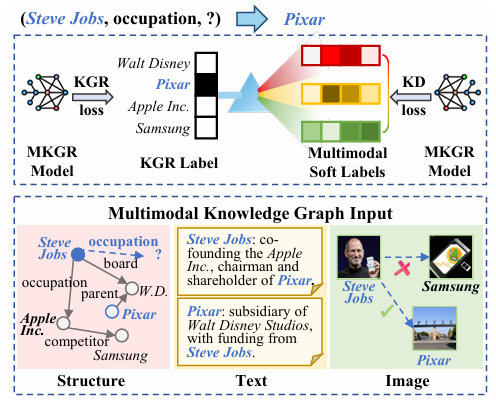
\includegraphics[width=\linewidth]{figures/fig1_dsom.png}
    \caption{Minh họa những hạn chế khi kết hợp các phương thức
    trong suy luận trên đồ thị tri thức đa phương thức và vai trò
    của tri thức từ phân phối dự đoán.  Nguồn: \cite{10.1145/3746027.3754576}, Hình 1.}
    \label{fig:dsom_motivation}
\end{figure}

Về tên của paper, nhóm hiểu tác giả đặt tên ``Dark Side of Modalities'' có nghĩa là sự ảnh hưởng tiêu cực khi một số phương thức có thể chứa thông tin nhiễu, không liên quan như phân tích ở đoạn đầu tiên. Và tác giả cũng định nghĩa ``Dark Knowlegde'' là tri thức ẩn trong phân phối dự đoán. Student không chỉ học đáp án đúng mà học cả phân phối logit từ teacher.

Nhóm phân tích cơ chế lựa chọn tổ hợp giáo viên RC theo bốn thành phần của học tăng cường: trạng thái, hành động, phần thưởng và chính sách.

\subsection{Phương pháp DSoM}

Kiến trúc tổng thể của DSoM được trình bày trong
Hình~\ref{fig:dsom_framework}. Phương pháp gồm
ba thành phần chính: xây dựng các mô hình giáo viên
theo từng phương thức, lựa chọn tổ hợp giáo viên
bằng học tăng cường và truyền tri thức sang mô hình
học sinh thông qua NDKD.

\begin{figure*}[t]
    \centering
    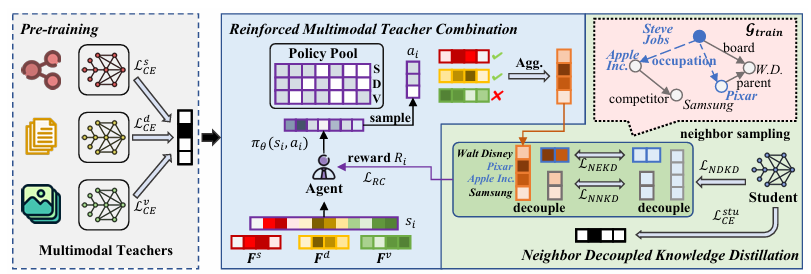
\includegraphics[width=\textwidth]{figures/fig2_dsom.png}
    \caption{Kiến trúc tổng thể DSoM gồm ba giai đoạn:
    huấn luyện các mô hình giáo viên theo từng phương thức,
    lựa chọn tổ hợp giáo viên bằng Reinforced Combination (RC)
    và truyền tri thức sang mô hình học sinh bằng
    Neighbor-Decoupled Knowledge Distillation (NDKD).
     Nguồn: \cite{10.1145/3746027.3754576}, Hình 2.}
    \label{fig:dsom_framework}
\end{figure*}


\subsubsection{Xây dựng các mô hình giáo viên và học sinh}

Để thực hiện Knowlegde Distillation, tác giả sẽ xây dựng các mô hình teacher và student. Trong paper, tác giả xây dựng ba teacher, mỗi teacher sẽ được học từ một nguồn phương thức tương ứng. Cụ thể là một teacher học từ thông tin cấu trúc (structure),
một teacher học thông tin từ hình ảnh (visual), và một teacher cuối học từ văn bản (textual). Các teacher được huấn luyện trước để dự đoán thực thể còn thiếu.  Theo cách hiểu của nhóm, việc phân chia như vậy giúp mô hình giữ lại được những góc nhìn khác nhau khi đánh giá cùng một truy vấn, thay vì kết hợp toàn bộ
thông tin ngay từ đầu.

Đối với các thông tin về hình ảnh và văn bản, tác giả sử dụng model pretrained như ViT và BERT để trích xuất đặc trưng. Các model này không trainable trong pipeline của DSoM mà chỉ tạo ra các vector đặc trưng ban đầu. Sau đó các vector đặc trưng này mới được đưa qua các lớp phép chiếu (projection layer) để model dự đoán thực thể còn thiếu. Các projection layer này có những tham số có thể học (trainable weights) trong quá trình huấn luyện teacher.

Xét một truy vấn $(h,r,?)$, mỗi teacher đều đưa
ra điểm dự đoán cho tất cả thực thể ứng viên trong tập
$E$. Ta ký hiệu kết quả của teacher thuộc phương thức
$m$ là:

\begin{equation}
F_m(h,r)=[f_m(h,r,e)]_{e\in E}.
\end{equation}

$f_m(h,r,e)$ là điểm của teacher $m$ đánh giá
mức độ phù hợp của thực thể $e$ với truy vấn $(h,r,?)$.
Kết quả mà teacher cho được không phải là
một thực thể được dự đoán, mà là một vector logits
chứa điểm của toàn bộ các thực thể ứng viên.

Các teacher sử dụng ComplEx để tính điểm dự đoán và
được huấn luyện với hàm loss là cross-entropy. Sau khi hoàn thành
huấn luyện, các logits của teacher được sử dụng để
hướng dẫn student.

Đối với student, tác giả sử dụng một mô hình chỉ học
embedding của thực thể và quan hệ từ cấu trúc
với hàm chấm điểm ComplEx tương tự như teacher. Điểm
khác biệt là student không trực tiếp sử dụng đặc trưng
hình ảnh hay văn bản.

Tác giả nói rằng việc lựa chọn mô hình student như vậy không đồng nghĩa với việc loại bỏ hoàn toàn thông tin đa phương thức, mà tác giả muốn truyền gián tiếp thông tin này qua quá trình distillation. Theo nhóm thì cách thiết kế này có lợi ích giảm sự phụ thuộc vào dữ liệu đa phương thức ở giai đoạn inference. Trong thực tế thì không phải thực thể nào cũng có đủ hình ảnh và văn bản mô tả đi kèm. 


\subsubsection{Lựa chọn tổ hợp giáo viên bằng học tăng cường}

Sau khi huấn luyện ba teacher, tác giả đề xuất
cơ chế Reinforced Combination (RC), sử dụng
học tăng cường (Reinforcement Learning - RL)
để lựa chọn và kết hợp các teacher phù hợp
với từng truy vấn.

Trong cơ chế này, agent không trực tiếp thực hiện bài toán MKGR, tức không dự đoán thực thể còn thiếu. Thay vào đó, agent quyết định những teacher nào sẽ tham gia hướng dẫn student thông qua quá trình Knowledge Distillation.


Để hiểu cách học tăng cường được áp dụng để chọn teacher hợp lý, nhóm phân tích bài toán qua các thành phần state,action, reward và policy.

\textit{a) Trạng thái (State):}


Agent cần có thông tin để quyết định nên lựa chọn teacher nào. Trạng thái trong DSoM được tạo bằng cach nối 3 vector logits của ba teacher:

\begin{equation}
s_i=[F_s\|F_v\|F_d].
\end{equation}

$F_s$, $F_v$ và $F_d$ lần lượt là logits
của teacher cấu trúc, hình ảnh và văn bản; ký hiệu
$\|$ biểu diễn phép nối vector.

Agent không trực tiếp nhận hình ảnh hay văn bản gốc. Thay vào đó, agent quan sát
kết quả dự đoán mà các teacher đưa ra. 

Nhóm thấy rằng cách thiết kế này hợp lý với mục tiêu
lựa chọn teacher. Vì thông tin cuối cùng được truyền
cho student chính là logits, nên agent sử dụng
logits để đánh giá sự khác biệt giữa các teacher
thay vì phải xử lý lại dữ liệu của từng phương thức.

\textit{b) Hành động (Action):}

Sau khi nhận trạng thái, agent phải quyết định sẽ
sử dụng những teacher nào.

Với ba teacher, mỗi teacher có hai khả năng là được
chọn hoặc không được chọn. Như vậy sẽ có $2^3=8$
tổ hợp, trừ đi một trường hợp không teacher nào được chọn, nên số hành động thực tế trong không gian
hành động của agent là:


\begin{equation}
|\mathcal{A}|=2^3-1=7.
\end{equation}

Ví dụ: Agent có thể lựa chọn riêng teacher
cấu trúc, kết hợp cấu trúc với văn bản, hoặc sử
dụng cả ba teacher,...

Tác giả sử dụng một mạng MLP để học phân phối xác
suất lựa chọn các tổ hợp này. Với trạng thái $s_i$,
agent lấy mẫu một hành động theo policy:

\begin{equation}
a_i\sim\pi_\theta(a\mid s_i).
\end{equation}




Sau khi xác định những teacher được chọn, tác giả lấy trung bình logits của chúng:

\begin{equation}
F_{\mathrm{tea}}^{(i)}
=
\frac{1}{|\mathcal{M}_i|}
\sum_{m\in\mathcal{M}_i}F_m^{(i)}.
\ 
\end{equation}

Trong đó, \(\mathcal{M}_i\) là tập teacher được agent lựa chọn cho mẫu huấn luyện thứ \(i\). Qua đối chiếu mã nguồn, agent thực hiện lựa chọn tổ hợp teacher riêng cho từng mẫu dữ liệu chứ không sử dụng một tổ hợp cố định cho toàn bộ batch. Nhiệm vụ của agent là học cách lựa chọn tổ hợp phù hợp, thay vì trực tiếp học trọng số kết hợp của từng teacher.

Sự khác biệt của phương pháp này so với cách kết hợp bằng trọng số là agent lựa chọn một trong bảy tổ hợp teacher có trước; và các teacher được chọn có trọng số bằng nhau. Chẳng hạn, nếu chọn Structure và Visual, DSoM sẽ lấy trung bình logits của hai teacher với trọng số là 0.5 và 0.5. Còn phương pháp kết hợp trọng số có thể học được giá trị như 0.75 và 0.25, nghĩa là structure đóng góp nhiều hơn visual. (Đã xác nhận điều này trong source code.)

\textit{c) Phần thưởng (Reward):}


Để biết một tổ hợp teacher được lựa chọn tốt hay không, nhóm sẽ trình bày
qua phần reward. Reward chính là tín hiệu dùng để đánh giá hành động của agent. Trong paper, tác giả sử dụng
Cross-Entropy để so sánh kết quả dự đoán của tổ hợp teacher với student:


\begin{equation}
R_i=
\begin{cases}
+1, & CE_{\mathrm{tea}}<CE_{\mathrm{stu}},\\
-10, & \text{ngược lại}.
\end{cases}
\end{equation}

$CE_{\mathrm{tea}}$ và $CE_{\mathrm{stu}}$
là Cross-Entropy của dự đoán từ tổ hợp teacher và
student đối với nhãn của mẫu đang xét.

Nếu tổ hợp teacher có Cross-Entropy thấp hơn student, agent được thưởng $+1$, ngược lại bị phạt $-10$. Vì student liên tục được cập nhật, cùng một tổ hợp teacher có thể nhận reward khác nhau trong quá trình huấn luyện.

Nhóm nhận thấy mức phạt lớn gấp mười lần mức thưởng, cho thấy tác giả muốn hạn chế việc lựa chọn những teacher dự đoán kém hơn student. Tuy nhiên, paper chưa giải thích rõ lý do lựa chọn hai giá trị $+1$ và $-10$ này.

Reward được tác giả tính bằng Cross-Entropy, chứ không trực tiếp sử dụng các
metric đánh giá MKGR như MRR hoặc Hits@K. Do đó,
agent đang học cách lựa chọn teacher dựa trên chất
lượng dự đoán theo Cross-Entropy, còn việc lựa chọn
này có cải thiện thứ hạng thực thể hay không cần
được đánh giá thực nghiệm.

\textit{d) Cập nhật chính sách (Policy):}


Sau khi nhận reward, agent sẽ cập nhật policy để những hành động có lợi có khả năng được chọn cao hơn trong các lần tiếp theo. Tác giả sử dụng Policy Gradient để cập nhật policy này. Ngoài reward của tổ hợp được chọn, mô hình còn xây dựng baseline bằng cách lấy trung bình logits của ba teacher rồi tính reward tương ứng.


Sự chênh lệch giữa reward của hành động và reward
baseline được ký hiệu:

\begin{equation}
\delta_i=R_i-\hat{R}_i.
\end{equation}

Ký hiệu $\hat{R}_i$ là phần thưởng baseline.
Giá trị $\delta_i$ được sử dụng khi cập nhật policy
để giảm phương sai của ước lượng gradient.

Hàm mất mát huấn luyện agent được viết:

\begin{equation}
\mathcal{L}_{RC}
=-\frac{1}{|\mathcal{T}_{train}|}
\sum_i \delta_i\log\pi_\theta(a_i\mid s_i).
\end{equation}

Nếu $\delta_i$ dương, việc tối thiểu hóa hàm mất
mát sẽ khuyến khích tăng xác suất của hành động
đã chọn. Ngược lại, khi $\delta_i$ âm, xác suất
của hành động đó sẽ bị giảm.

Toàn bộ quá trình RL trong DSoM có thể
được hiểu như sau: agent nhận các logits của ba
teacher, lựa chọn một tổ hợp, sử dụng kết quả tổ
hợp để tính reward, sau đó cập nhật policy. Agent không học cách trả
lời trực tiếp truy vấn $(h,r,?)$, mà học cách
lựa chọn nguồn tri thức để hỗ trợ student.

\subsubsection{Neighbor-Decoupled Knowledge Distillation}


Agent đã lựa chọn teacher và tạo ra logits tổng hợp, bước tiếp theo là chuyển những thông tin này sang student. Nếu chỉ lấy thực thể có điểm dự đoán cao nhất từ teacher làm nhãn huấn luyện, student sẽ không học được toàn bộ thông tin trong phân phối dự đoán. Tác giả sử dụng Knowledge Distillation cũng chính vì muốn student học được thông tin trong phân phối dự đoán này.


Logits của teacher và student được
chuyển thành phân phối xác suất thông qua softmax
với tham số nhiệt độ (temperature) $\tau$:

\begin{equation}
\begin{aligned}
P_{\mathrm{tea}}&=
\operatorname{softmax}(F_{\mathrm{tea}}/\tau),\\
P_{\mathrm{stu}}&=
\operatorname{softmax}(F_{\mathrm{stu}}/\tau).
\end{aligned}
\end{equation}








Trong MKGR, một truy vấn có thể có nhiều đáp án đúng. Ví dụ với truy vấn $(A,r,?)$, nếu đồ thị tồn tại hai bộ ba $(A,r,B)$ và $(A,r,C)$ thì cả $B$ và $C$ đều là đáp án đúng. Nếu chỉ xét bộ ba $(A,r,B)$, thực thể $C$ có thể bị xem là một đáp án không đúng, mặc dù nó cũng có quan hệ $r$ với $A$.

Trong Knowledge Distillation, phương pháp Decoupled Knowledge Distillation (DKD) phân tách việc học thành thông tin của nhãn đích và các nhãn còn lại. Tuy nhiên, cách phân tách này chưa phù hợp với đặc điểm nhiều đáp án đúng của MKGR. Vì vậy, tác giả đề xuất Neighbor-Decoupled Knowledge Distillation (NDKD), trong đó thay vì chỉ xét một đáp án đúng, mô hình xét toàn bộ tập neighbors:

\[
\mathcal{N}(h,r)=
\{e\mid(h,r,e)\in\mathcal{T}_{train}\}.
\]

Đây là tập các thực thể có quan hệ $r$ với $h$ trong tập huấn luyện. Những thực thể không thuộc tập này được gọi là non-neighbors.

Nhóm lưu ý rằng non-neighbors không nhất thiết
là những đáp án sai trong thế giới thực. Do KG
có thể chưa hoàn chỉnh, một thực thể không có
trong tập neighbors chỉ có nghĩa quan hệ tương
ứng chưa được ghi nhận trong dữ liệu đang xét.

Sau khi chia các thực thể thành hai nhóm, tác
giả xây dựng hai thành phần loss.










\textit{a) Neighbor Entity Knowledge Distillation (NEKD):}

Thành phần NEKD giúp student học cách teacher đánh giá nhóm neighbors, thay vì chỉ tập trung vào một đáp án đúng.

Chẳng hạn, với truy vấn $(A,r,?)$, giả sử $B$ và $C$ là hai neighbors. Teacher dự đoán xác suất của $B$ và $C$ lần lượt là $0.4$ và $0.3$, trong khi student dự đoán $0.2$ và $0.1$.

Theo công thức trong paper, tác giả lấy trung bình xác suất của các neighbors:

\begin{equation}
p_{\mathcal{N}}=
\frac{1}{|\mathcal{N}|}
\sum_{e\in\mathcal{N}}p_e.
\label{eq:nekd_mean}
\end{equation}

Với ví dụ trên, teacher có xác suất trung bình là $0.35$, còn student là $0.15$. Từ đó, tác giả tạo hai phân phối nhị phân:

\begin{equation}
\begin{aligned}
b_{\mathrm{tea}}&=[0.35,0.65],\\
b_{\mathrm{stu}}&=[0.15,0.85].
\end{aligned}
\end{equation}

Hai phân phối này được so sánh bằng KL Divergence:

\begin{equation}
\mathcal{L}_{NEKD}
=KL(b_{\mathrm{tea}}\|b_{\mathrm{stu}}).
\end{equation}

NEKD giúp student điều chỉnh xác suất dành cho nhóm neighbors sao cho gần với teacher hơn.

Công thức~\eqref{eq:nekd_mean} và ví dụ trên trình bày
cách lấy trung bình xác suất của các thực thể thuộc nhóm
neighbors theo bài báo gốc. Tuy nhiên, theo tài liệu giao thức
thực nghiệm của repository, mã nguồn được sử dụng trong
các lần tái lập tính xác suất nhóm neighbors bằng phép tổng:

\begin{equation}
    p_N^{\mathrm{impl}} = \sum_{e \in N} p_e,
    \label{eq:nekd_sum}
\end{equation}

\noindent
sau đó xây dựng phân phối nhị phân
$\left[p_N^{\mathrm{impl}},\,1-p_N^{\mathrm{impl}}\right]$.
Hai cách tính khác nhau khi tập neighbors có nhiều hơn
một phần tử. Do đó, cần phân biệt công thức trình bày
theo bài báo với cách triển khai thực tế được sử dụng
để tạo ra các kết quả tái lập.

Một vấn đề mà nhóm nhận ra ở đây là phân phối xác suất của các neighbors được đại diện bởi một giá trị trung bình, nên có thể làm mất thông tin về xác suất của từng thực thể. Ví dụ 1 tập neighbor là $\{A,B,C\}$ có 3 phần tử, teacher dự đoán $[0.3,0.2,0.1]$ và student dự đoán $[0.1,0.3,0.2]$ vẫn cho NEKD loss bằng $0$ (vì trung bình cả hai đều là $0.2$), mặc dù xác suất của từng neighbor khác nhau. Tuy nhiên, điều này chưa hẳn là hạn chế, vì các neighbors đều là đáp án đúng và không nhất thiết phải có cùng thứ tự ưu tiên.

\textit{b) Non-Neighbor Knowledge Distillation
(NNKD):}

Thành phần thứ hai tập trung vào các thực thể không thuộc tập neighbors.

Tác giả chuẩn hóa lại xác suất của những thực thể non-neighbors để tạo thành một phân phối riêng:

\begin{equation}
\tilde{p}_e=
\frac{p_e}
{\sum_{j\notin\mathcal{N}}p_j},
\quad e\notin\mathcal{N}.
\end{equation}

Sau đó student được hướng dẫn học phân phối này từ teacher thông qua:

\begin{equation}
\mathcal{L}_{NNKD}
=KL(\widetilde{P}_{\mathrm{tea}}
\|\widetilde{P}_{\mathrm{stu}}).
\end{equation}

Đây là thành phần thể hiện khá rõ
ý tưởng Dark Knowledge của tác giả.

Ví dụ, trong tập non-neighbors có ba thực thể
$\{D,E,F\}$. Mặc dù cả ba đều không thuộc
tập đáp án đúng đã biết, teacher có thể đánh
giá $D$ phù hợp với truy vấn hơn $E$, và $E$
phù hợp hơn $F$.

Nếu chỉ học nhãn đúng hoặc sai, student không
nhận được đầy đủ những thông tin này. Nhưng
khi học phân phối của teacher, student có thể
học thêm mức độ phù hợp tương đối giữa các
thực thể không phải đáp án đích.

NNKD không cần khẳng định các non-neighbors đều thực sự
sai. Thành phần này khai thác sự khác biệt
trong cách teacher đánh giá những thực thể
chưa được ghi nhận là đáp án đúng.

Cuối cùng, hai thành phần được kết hợp:

\begin{equation}
\mathcal{L}_{NDKD}
=\alpha\mathcal{L}_{NEKD}
+\beta\mathcal{L}_{NNKD}.
\end{equation}

$\alpha$ và $\beta$ là các hệ số điều chỉnh đóng góp của từng thành phần.

Đóng góp chính của NDKD không phải là việc sử dụng KL Divergence (kỹ
thuật này đã phổ biến trong Knowledge Distillation) mà là điều chỉnh
cách phân tách phân phối xác suất để phù hợp
với trường hợp một truy vấn có nhiều đáp án
đúng trong MKGR.

Nhóm cho rằng hiệu quả của
cách phân tách này phụ thuộc vào chất lượng
của tập neighbors được ghi nhận. Nếu dữ liệu
huấn luyện còn thiếu nhiều quan hệ, một số
đáp án thực sự đúng vẫn có thể bị đưa vào
tập non-neighbors.

\subsubsection{Hàm mất mát và quy trình huấn luyện}

Sau khi phân tích hai thành phần trên, nhóm
tổng hợp lại quy trình huấn luyện của DSoM.

Đầu tiên, ba teacher được huấn luyện trước,
mỗi teacher khai thác một phương thức khác
nhau. Sau đó, student được khởi tạo để học
từ nhãn thực tế của bài toán MKGR và từ
phân phối dự đoán của các teacher.

Trong quá trình huấn luyện student, agent
nhận logits từ ba teacher để lựa chọn tổ
hợp phù hợp. Các logits được chọn được lấy
trung bình số lượng teacher trong tổ hợp, sau đó sử dụng trong NDKD để
hướng dẫn student.

Đồng thời, agent nhận reward từ việc so
sánh Cross-Entropy giữa tổ hợp teacher
và student để cập nhật policy của mình.

Hàm mục tiêu tổng thể trong paper là:

\begin{equation}
\mathcal{L}_{stu}
=\mathcal{L}^{stu}_{CE}
+\mathcal{L}_{RC}
+\gamma\mathcal{L}_{NDKD}.
\end{equation}

Trong đó, $\mathcal{L}^{stu}_{CE}$ là loss
dự đoán thực thể của student,
$\mathcal{L}_{RC}$ là loss của agent và
$\mathcal{L}_{NDKD}$ là loss dùng để truyền
tri thức từ teacher sang student. Hệ số
$\gamma$ điều chỉnh mức đóng góp của NDKD.

Dù được viết chung trong hàm mục tiêu, các thành phần
này đảm nhận những nhiệm vụ khác nhau.
Loss của agent dùng để học chính sách lựa
chọn teacher, còn Cross-Entropy và NDKD
được sử dụng để huấn luyện student.

Cuối cùng, ở giai đoạn inference, tác giả
chỉ sử dụng student. Các teacher và agent
không còn tham gia vào việc dự đoán thực
thể còn thiếu.

Như vậy, theo cách hiểu của nhóm, DSoM
có thể được nhìn nhận qua hai câu hỏi:
student nên học từ những teacher nào,
và student nên học những thông tin gì
từ kết quả dự đoán của các teacher đó?

Reinforced Teacher Combination giải quyết
câu hỏi thứ nhất thông qua học tăng cường,
còn NDKD giải quyết câu hỏi thứ hai thông
qua việc phân tách phân phối dự đoán.

Đây cũng là hai thành phần mà nhóm cho
rằng thể hiện rõ nhất ý tưởng của tác giả
trong công trình DSoM.

\subsection{Tái lập thực nghiệm}

\subsubsection{Thiết lập thực nghiệm}

Nhóm sử dụng mã nguồn công khai của DSoM và bổ sung các script chuẩn bị dữ liệu (vì code do tác giả công bố bị thiếu nhiều thành phần liên quan đến chuẩn bị dataset, các hàm phụ trợ,...). Nhóm đánh giá và theo dõi kết quả bằng W\&B.
Mã nguồn tái lập được công bố tại
\href{https://github.com/keiranoluv/Reproduce_DSoM}{GitHub}.

Thực nghiệm được thực hiện trên GPU NVIDIA
GeForce RTX 5090, Python 3.12,
PyTorch 2.7.0 (CUDA 12.8), với random seed 2022.
Cấu hình chính gồm rank 2000, batch size 1000,
optimizer Adagrad với learning rate 0.1,
regularization N3 bằng 0.01, tối đa 200 epochs,
validation mỗi 3 epochs và early stopping
patience 10. Student sử dụng KD temperature 4,
trọng số KD bằng 2 và $\alpha=\beta=1$.

Nhóm tái lập trên sáu bộ dữ liệu gồm DB15K,
MKG-W, MKG-Y, FB15K-237, WN18 và WN9.
Teacher sử dụng thông tin cấu trúc, hình ảnh
và văn bản, trong khi student chỉ sử dụng
thông tin cấu trúc. Các đặc trưng hình ảnh
và văn bản được tái tạo bằng ViT và BERT.

Nhóm bổ sung pipeline trích xuất đặc trưng ảnh do mã nguồn công
khai chưa cung cấp script tương ứng. Tuy nhiên, pipeline tái lập
sử dụng đầu vào $384\times384$, khác với cấu hình
\texttt{vit-base-patch16-224} được tác giả công bố.
Đây là sai khác trong triển khai của nhóm; ảnh hưởng đến kết quả
chưa được định lượng.

Checkpoint của teacher được chọn theo
validation Hits@10, còn checkpoint của
student được chọn theo validation MRR.
Các kết quả test được lấy từ
\texttt{final\_result} của checkpoint
được chọn thay vì metric ở epoch cuối.

Giới hạn về dữ liệu: Tập validation của DB15K trong nguồn dữ liệu công khai có các bộ ba trùng với tập huấn luyện và tập kiểm tra. Nhóm giữ nguyên cách chia dữ liệu này trong các thực nghiệm đối chiếu. Do validation được sử dụng để chọn checkpoint, sự trùng lặp làm giảm tính độc lập của quá trình lựa chọn mô hình và có thể khiến kết quả đánh giá lạc quan hơn. Vì vậy, các kết quả trên DB15K cần được diễn giải cùng giới hạn này.

Nhóm sử dụng ba chế độ thực nghiệm:

\begin{itemize}
    % \item \texttt{source\_frozen}: Giữ nguyên mã nguồn công khai tác giả công bố. Vấn đề trong mã nguồn này là agent có lựa chọn tổ hợp teacher nhưng policy không được cập nhật do thiếu tham số trong optimizer - đây là điểm không khớp giữa paper và mã nguồn.
    \item \texttt{source\_frozen}: giữ cách cập nhật tham số của mã nguồn
        công khai DSoM tại commit \texttt{171e59c}. Policy vẫn nhận
        logits của teacher và lấy mẫu tổ hợp bằng
        \texttt{torch.multinomial}.
        \footnote{\href{https://github.com/OreOZhao/DSoM/blob/171e59cb069d50abf039fa824b079e23b8956696/src/kd.py\#L337-L354}{DSoM: tính phân phối policy và lấy mẫu tổ hợp.}}
        Tuy nhiên, \texttt{get\_learnable\_parameters} chỉ trả về tham
        số student, còn optimizer được khởi tạo từ danh sách này,
        nên tham số mạng policy không được cập nhật.
        \footnote{\href{https://github.com/OreOZhao/DSoM/blob/171e59cb069d50abf039fa824b079e23b8956696/src/kd.py\#L22-L24}{DSoM: danh sách tham số được tối ưu};
        \href{https://github.com/OreOZhao/DSoM/blob/171e59cb069d50abf039fa824b079e23b8956696/src/kd_learn.py\#L246-L255}{khởi tạo optimizer}.}
        Do đó, ``frozen'' chỉ việc giữ nguyên tham số policy, không
        đồng nghĩa luôn chọn một tổ hợp teacher cố định. Các kết quả
        này chưa chứng minh hiệu quả của việc học policy bằng RL.
    \item \texttt{learned\_RC}: Bổ sung optimizer riêng để huấn luyện policy theo cơ chế RL giống mô tả của paper;
    \item \texttt{fixed\_teacher}: Sử dụng một teacher hoặc tổ hợp cố định, không qua agent. Sự phân biệt này giúp đánh giá riêng khả năng tái lập mã nguồn và hiệu quả của cơ chế RL được đề xuất trong paper.
\end{itemize}

Để đánh giá khả năng tái lập và kiểm chứng
các thành phần của DSoM, nhóm tổ chức
thực nghiệm theo Bảng~\ref{tab:dsom_exp_overview}.

\begin{table}[htbp]
\centering
\caption{Tổng quan các nhóm thực nghiệm DSoM.}
\label{tab:dsom_exp_overview}
\scriptsize
\setlength{\tabcolsep}{3pt}
\renewcommand{\arraystretch}{1.2}

\begin{tabular}{@{}
>{\raggedright\arraybackslash}p{0.27\columnwidth}
>{\raggedright\arraybackslash}p{0.45\columnwidth}
>{\raggedright\arraybackslash}p{0.20\columnwidth}@{}}

\toprule
\textbf{Thực nghiệm}
& \textbf{Mục tiêu}
& \textbf{Bảng đối chiếu so với paper} \\
\midrule

Benchmark
& Đối chiếu chất lượng dự đoán trên
sáu bộ dữ liệu.
& Tables 1, 3, 7 \\

\addlinespace
Teacher selection
& So sánh các chiến lược
lựa chọn teacher.
& Table 2 \\

\addlinespace
Component ablation
& Đánh giá vai trò của RC,
NEKD và NNKD.
& Table 4 \\

\addlinespace
Modality ablation
& Đánh giá đóng góp của từng
nguồn thông tin.
& Table 6 \\


\bottomrule
\end{tabular}
\end{table}




Nhóm còn thực hiện các thí nghiệm bổ sung
Exp01 và A1-A10 trên DB15K nhằm phân tích
sâu hơn vai trò của teacher selection và
distillation.


\providecolor{resultgray}{gray}{0.94}
\providecommand{\dsomrunbase}{https://forge.coreweave.com/wandb/keiranoluv-hcmus/DSoM-Reproduction/runs/}
\providecommand{\dsomreprocell}[1]{\cellcolor{resultgray}#1}
\providecommand{\dsomrun}[2]{\cellcolor{resultgray}\href{\dsomrunbase#1}{#2}}
\providecommand{\dsomsource}[2]{\cellcolor{resultgray}\href{\dsomrunbase#1}{#2}\textsuperscript{\textdagger}}
\providecommand{\dsomlink}[2]{\href{\dsomrunbase#1}{#2}}
\providecommand{\deltaneg}[1]{\textcolor{red!70!black}{#1}}
\providecommand{\deltapos}[1]{\textcolor{green!45!black}{#1}}



\subsubsection{Kết quả và phân tích}

\par\noindent\hspace{0pt}
\begingroup
\raggedbottom
\setlength{\intextsep}{7pt plus 0pt minus 2pt}

\noindent\textit{Quy ước chung cho các bảng:}
$\uparrow$ biểu thị chỉ số càng cao càng tốt;
$\downarrow$ biểu thị chỉ số càng thấp càng tốt.
MRR và Hits@K tính theo \%, MR tính theo thứ hạng trung bình.
$\Delta$ là chênh lệch giữa kết quả tái lập và kết quả được công bố trong paper, chỉ số
\textcolor{green!45!black}{xanh} là cải thiện,
\textcolor{red!70!black}{đỏ} là suy giảm.
Các ô nền xám liên kết tới run W\&B; kết quả student
lấy từ checkpoint được chọn theo validation MRR.


\noindent\textit{Khả năng tái lập kết quả tổng thể:}
Nhóm tái lập kết quả của student và so sánh với paper trên
sáu bộ dữ liệu. Các kết quả được so sánh với Tables 1, 3 và 7 trong paper,
với baseline tái lập sử dụng \texttt{source\_frozen} RC, nghĩa là sử dụng lại mã nguồn của tác giả mà không chỉnh sửa những sai khác so với các phương pháp được nêu trong paper.

Trên DB15K, MRR tái lập thấp hơn paper 1.38 \%;
MKG-W chỉ lệch -0.32 \%, còn MKG-Y cao hơn
paper 0.67\% (Bảng~\ref{tab:dsom_mmkg}).


\begin{table}[H]
\centering
\caption{So sánh MRR và Hits@K trên \\ DB15K, MKG-W và MKG-Y (Table 1 trong paper).}
\label{tab:dsom_mmkg}
\scriptsize
\setlength{\tabcolsep}{3pt}
\renewcommand{\arraystretch}{1.12}
\begin{tabular}{@{}llrrrr@{}}
\toprule
\textbf{Dataset} & \textbf{Nguồn} & \textbf{MRR$\uparrow$} & \textbf{H@1$\uparrow$} & \textbf{H@3$\uparrow$} & \textbf{H@10$\uparrow$} \\
\midrule
DB15K & Paper & 42.68 & 34.45 & 46.62 & 58.12 \\
 & \dsomreprocell{Tái lập} & \dsomrun{gvpp95st}{41.30} & \dsomrun{gvpp95st}{33.17} & \dsomrun{gvpp95st}{45.47} & \dsomrun{gvpp95st}{56.57} \\
 & $\Delta$ & \deltaneg{-1.38} & \deltaneg{-1.28} & \deltaneg{-1.15} & \deltaneg{-1.55} \\
\addlinespace
MKG-W & Paper & 40.90 & 33.56 & 43.58 & 55.28 \\
 & \dsomreprocell{Tái lập} & \dsomrun{530tgh0o}{40.58} & \dsomrun{530tgh0o}{33.54} & \dsomrun{530tgh0o}{43.19} & \dsomrun{530tgh0o}{53.73} \\
 & $\Delta$ & \deltaneg{-0.32} & \deltaneg{-0.02} & \deltaneg{-0.39} & \deltaneg{-1.55} \\
\addlinespace
MKG-Y & Paper & 40.02 & 35.67 & 41.70 & 47.71 \\
 & \dsomreprocell{Tái lập} & \dsomrun{2a9t5tjk}{40.69} & \dsomrun{2a9t5tjk}{36.01} & \dsomrun{2a9t5tjk}{42.41} & \dsomrun{2a9t5tjk}{48.99} \\
 & $\Delta$ & \deltapos{+0.67} & \deltapos{+0.34} & \deltapos{+0.71} & \deltapos{+1.28} \\
\addlinespace
\bottomrule
\end{tabular}

\end{table}


Với FB15K-237, các chỉ số Hits@K chênh lệch không quá
0.29\% theo giá trị tuyệt đối. Trên WN18,
Hits@10 thấp hơn paper 0.51\%
(Bảng~\ref{tab:dsom_kg}).


\begin{table}[H]
\centering
\caption{Kết quả trên FB15K-237 và WN18 (Table 3 trong paper).}
\label{tab:dsom_kg}
\scriptsize
\setlength{\tabcolsep}{3pt}
\renewcommand{\arraystretch}{1.12}
\begin{tabular}{@{}llrrrr@{}}
\toprule
\textbf{Dataset} & \textbf{Nguồn} & \textbf{MR$\downarrow$} & \textbf{H@1$\uparrow$} & \textbf{H@3$\uparrow$} & \textbf{H@10$\uparrow$} \\
\midrule
FB15K-237 & Paper & 116.00 & 27.50 & 41.10 & 56.40 \\
 & \dsomreprocell{Tái lập} & \dsomrun{pebphkp6}{116.56} & \dsomrun{pebphkp6}{27.79} & \dsomrun{pebphkp6}{41.05} & \dsomrun{pebphkp6}{56.67} \\
 & $\Delta$ & \deltaneg{+0.56} & \deltapos{+0.29} & \deltaneg{-0.05} & \deltapos{+0.27} \\
\addlinespace
WN18 & Paper & 7.00 & 95.00 & 96.20 & 97.40 \\
 & \dsomreprocell{Tái lập} & \dsomrun{otquhagi}{8.96} & \dsomrun{otquhagi}{94.87} & \dsomrun{otquhagi}{95.92} & \dsomrun{otquhagi}{96.89} \\
 & $\Delta$ & \deltaneg{+1.96} & \deltaneg{-0.13} & \deltaneg{-0.28} & \deltaneg{-0.51} \\
\addlinespace
\bottomrule
\end{tabular}

\end{table}




Trên WN9, kết quả tái lập theo giao thức filtered đạt MRR
91.96\%, so với 92.13\% trong bài báo. Mục~5.1 của bài báo
công bố sử dụng filtered để loại các đáp án đúng khác trước khi
tính thứ hạng; phần trình bày WN9 không nêu ngoại lệ.
Khi đánh giá raw trên cùng checkpoint được chọn bằng validation
MRR theo filtered, MRR đạt 61.88\%. Nhóm dùng filtered để đối
chiếu với giao thức được công bố và báo thêm raw nhằm minh họa
ảnh hưởng của cách đánh giá. Sự gần nhau về số liệu chưa đủ chứng
minh toàn bộ dữ liệu và chi tiết triển khai của hai bên tương đương.
Bảng~\ref{tab:dsom_wn9} trình bày kết quả theo cả hai giao thức.


\begin{table}[H]
\centering
\caption{Kết quả DSoM trên WN9 (Table 7).}
\label{tab:dsom_wn9}
\scriptsize
\setlength{\tabcolsep}{3pt}
\renewcommand{\arraystretch}{1.12}
\begin{tabular}{@{}lrrrr@{}}
\toprule
\textbf{Nguồn} & \textbf{MRR$\uparrow$} & \textbf{H@1$\uparrow$} & \textbf{H@3$\uparrow$} & \textbf{H@10$\uparrow$} \\
\midrule
Paper & 92.13 & 90.52 & -- & 95.56 \\
\dsomreprocell{Tái lập (filtered)} & \dsomrun{8k36o3o8}{91.96} & \dsomrun{8k36o3o8}{90.33} & \dsomrun{8k36o3o8}{92.84} & \dsomrun{8k36o3o8}{94.96} \\
$\Delta$ (filtered) & \deltaneg{-0.17} & \deltaneg{-0.19} & -- & \deltaneg{-0.60} \\
\addlinespace
\dsomreprocell{Tái lập (raw)} & \dsomsource{8k36o3o8}{61.88} & \dsomsource{8k36o3o8}{52.05} & \dsomsource{8k36o3o8}{66.94} & \dsomsource{8k36o3o8}{81.01} \\
\bottomrule
\end{tabular}

\par\smallskip
\begin{minipage}{0.98\linewidth}
\scriptsize
\textit{Raw}: Xếp hạng trên toàn bộ thực thể ứng viên,
kể cả các đáp án đúng khác đã biết.
\textit{Filtered}: Loại các đáp án đúng khác
đã biết trước khi tính thứ hạng.

\textsuperscript{\textdagger}
Raw được nhóm đánh giá bổ sung trên cùng
checkpoint (epoch 15); liên kết W\&B
dẫn đến run huấn luyện.
\end{minipage}
\end{table}



\noindent\textit{Ảnh hưởng của cách lựa chọn teacher:}
Nhóm tái lập Table 2 trong paper nhằm so sánh
các phương pháp lựa chọn teacher trên ba bộ dữ liệu
DB15K, MKG-W và MKG-Y (Bảng~\ref{tab:dsom_table2_combined}).

ConfTeacher chọn teacher có xác suất softmax cao nhất;
BestTeacher chọn teacher có Cross-Entropy (CE)
thấp nhất; BestStrategy chọn tổ hợp có CE thấp nhất
trong bảy tổ hợp. Riêng MulDE là phương pháp
distillation sử dụng nhiều teacher, được nhóm
điều chỉnh để phù hợp với framework DSoM
do thiếu thông tin tương ứng trong mã nguồn và paper.

\begin{table*}[!t]
\centering
\caption{So sánh các phương pháp teacher selection trên DB15K, MKG-W và MKG-Y (Table 2 trong paper).}
\label{tab:dsom_table2_combined}
\begingroup
\fontsize{8}{9.3}\selectfont
\setlength{\tabcolsep}{2.2pt}
\renewcommand{\arraystretch}{1.04}
\begin{tabular}{@{}ll*{12}{r}@{}}
\toprule
\textbf{Phương pháp} & \textbf{Nguồn} & \multicolumn{4}{c}{\textbf{DB15K}} & \multicolumn{4}{c}{\textbf{MKG-W}} & \multicolumn{4}{c}{\textbf{MKG-Y}} \\
\cmidrule(lr){3-6}\cmidrule(lr){7-10}\cmidrule(l){11-14}
& & \textbf{MRR$\uparrow$} & \textbf{H@1$\uparrow$} & \textbf{H@3$\uparrow$} & \textbf{H@10$\uparrow$} & \textbf{MRR$\uparrow$} & \textbf{H@1$\uparrow$} & \textbf{H@3$\uparrow$} & \textbf{H@10$\uparrow$} & \textbf{MRR$\uparrow$} & \textbf{H@1$\uparrow$} & \textbf{H@3$\uparrow$} & \textbf{H@10$\uparrow$} \\
\midrule
DSoM & Paper & 42.68 & 34.45 & 46.62 & 58.12 & 40.90 & 33.56 & 43.58 & 55.28 & 40.02 & 35.67 & 41.70 & 47.71 \\
 & \dsomreprocell{Tái lập} & \dsomrun{gvpp95st}{41.30} & \dsomrun{gvpp95st}{33.17} & \dsomrun{gvpp95st}{45.47} & \dsomrun{gvpp95st}{56.57} & \dsomrun{530tgh0o}{40.58} & \dsomrun{530tgh0o}{33.54} & \dsomrun{530tgh0o}{43.19} & \dsomrun{530tgh0o}{53.73} & \dsomrun{2a9t5tjk}{40.69} & \dsomrun{2a9t5tjk}{36.01} & \dsomrun{2a9t5tjk}{42.41} & \dsomrun{2a9t5tjk}{48.99} \\
 & $\Delta$ & \deltaneg{-1.38} & \deltaneg{-1.28} & \deltaneg{-1.15} & \deltaneg{-1.55} & \deltaneg{-0.32} & \deltaneg{-0.02} & \deltaneg{-0.39} & \deltaneg{-1.55} & \deltapos{+0.67} & \deltapos{+0.34} & \deltapos{+0.71} & \deltapos{+1.28} \\
\addlinespace[2.5pt]
ConfTeacher & Paper & 40.87 & 32.82 & 44.75 & 56.16 & 37.49 & 31.50 & 39.64 & 48.97 & 37.76 & 33.93 & 39.82 & 44.24 \\
 & \dsomreprocell{Tái lập} & \dsomrun{sa6dphy6}{40.81} & \dsomrun{sa6dphy6}{32.96} & \dsomrun{sa6dphy6}{44.66} & \dsomrun{sa6dphy6}{55.82} & \dsomrun{ipotae21}{37.72} & \dsomrun{ipotae21}{31.83} & \dsomrun{ipotae21}{39.87} & \dsomrun{ipotae21}{49.18} & \dsomrun{69whpbut}{38.60} & \dsomrun{69whpbut}{35.02} & \dsomrun{69whpbut}{40.16} & \dsomrun{69whpbut}{45.21} \\
 & $\Delta$ & \deltaneg{-0.06} & \deltapos{+0.14} & \deltaneg{-0.09} & \deltaneg{-0.34} & \deltapos{+0.23} & \deltapos{+0.33} & \deltapos{+0.23} & \deltapos{+0.21} & \deltapos{+0.84} & \deltapos{+1.09} & \deltapos{+0.34} & \deltapos{+0.97} \\
\addlinespace[2.5pt]
BestTeacher & Paper & 41.43 & 33.46 & 45.40 & 56.56 & 38.27 & 32.41 & 40.48 & 49.61 & 38.51 & 34.89 & 40.39 & 44.71 \\
 & \dsomreprocell{Tái lập} & \dsomrun{7h7gppby}{40.97} & \dsomrun{7h7gppby}{32.95} & \dsomrun{7h7gppby}{44.89} & \dsomrun{7h7gppby}{56.36} & \dsomrun{4j77nc0v}{37.73} & \dsomrun{4j77nc0v}{31.68} & \dsomrun{4j77nc0v}{40.29} & \dsomrun{4j77nc0v}{48.91} & \dsomrun{pde7aget}{38.72} & \dsomrun{pde7aget}{35.09} & \dsomrun{pde7aget}{40.44} & \dsomrun{pde7aget}{45.02} \\
 & $\Delta$ & \deltaneg{-0.46} & \deltaneg{-0.51} & \deltaneg{-0.51} & \deltaneg{-0.20} & \deltaneg{-0.54} & \deltaneg{-0.73} & \deltaneg{-0.19} & \deltaneg{-0.70} & \deltapos{+0.21} & \deltapos{+0.20} & \deltapos{+0.05} & \deltapos{+0.31} \\
\addlinespace[2.5pt]
BestStrategy & Paper & 41.65 & 33.60 & 45.81 & 56.94 & 39.14 & 32.88 & 41.55 & 51.10 & 39.34 & 35.58 & 41.01 & 45.74 \\
 & \dsomreprocell{Tái lập} & \dsomrun{7jui1jln}{41.53} & \dsomrun{7jui1jln}{33.66} & \dsomrun{7jui1jln}{45.45} & \dsomrun{7jui1jln}{56.54} & \dsomrun{x2xnt5dv}{38.21} & \dsomrun{x2xnt5dv}{32.01} & \dsomrun{x2xnt5dv}{40.52} & \dsomrun{x2xnt5dv}{49.74} & \dsomrun{ig4dosz9}{38.90} & \dsomrun{ig4dosz9}{34.74} & \dsomrun{ig4dosz9}{41.12} & \dsomrun{ig4dosz9}{45.98} \\
 & $\Delta$ & \deltaneg{-0.12} & \deltapos{+0.06} & \deltaneg{-0.36} & \deltaneg{-0.40} & \deltaneg{-0.93} & \deltaneg{-0.87} & \deltaneg{-1.03} & \deltaneg{-1.36} & \deltaneg{-0.44} & \deltaneg{-0.84} & \deltapos{+0.11} & \deltapos{+0.24} \\
\addlinespace[2.5pt]
MulDE & Paper & 39.94 & 31.74 & 43.52 & 56.03 & 38.68 & 32.39 & 41.11 & 50.36 & 39.62 & 35.60 & 41.19 & 46.68 \\
 & \dsomreprocell{Tái lập\textsuperscript{\textdagger}} & \dsomrun{21cexx1p}{38.79} & \dsomrun{21cexx1p}{31.64} & \dsomrun{21cexx1p}{42.39} & \dsomrun{21cexx1p}{52.34} & \dsomrun{s0ob59f5}{37.32} & \dsomrun{s0ob59f5}{31.07} & \dsomrun{s0ob59f5}{39.47} & \dsomrun{s0ob59f5}{49.31} & \dsomrun{s763om5u}{39.00} & \dsomrun{s763om5u}{34.59} & \dsomrun{s763om5u}{40.89} & \dsomrun{s763om5u}{46.40} \\
 & $\Delta$ & \deltaneg{-1.15} & \deltaneg{-0.10} & \deltaneg{-1.13} & \deltaneg{-3.69} & \deltaneg{-1.36} & \deltaneg{-1.32} & \deltaneg{-1.64} & \deltaneg{-1.05} & \deltaneg{-0.62} & \deltaneg{-1.01} & \deltaneg{-0.30} & \deltaneg{-0.28} \\
\bottomrule
\end{tabular}
\endgroup
\par\smallskip
{\scriptsize DSoM tái lập dùng \texttt{source\_frozen} RC; ConfTeacher/BestTeacher/BestStrategy dùng NDKD. \textsuperscript{\textdagger}MulDE tái lập là bản điều chỉnh sử dụng Senior và KL; \\ chưa xác nhận trùng cấu hình MulDE trong paper.}
\end{table*}

Trên DB15K, BestStrategy đạt MRR 41.53\%, cao hơn
DSoM source-frozen RC (41.30\%). Ngược lại, DSoM
source-frozen có MRR cao nhất trong các phương pháp
đã chạy trên MKG-W và MKG-Y. Do policy của baseline
source-frozen không được cập nhật, kết quả Table 2
chưa đủ khẳng định hiệu quả của RL như mô tả trong paper.

\noindent\textit{Đóng góp của các thành phần:}
Nhóm đối chiếu thí nghiệm ablation trong Table 4 nhằm
kiểm tra vai trò của cơ chế lựa chọn teacher (RC) và
các hàm distillation. Ba cấu hình đầu đánh giá trực tiếp
teacher hoặc tổ hợp teacher; các cấu hình còn lại huấn luyện
student. Kết quả Paper và Tái lập được trình bày cạnh nhau
trong Bảng~\ref{tab:dsom_table4}.

\begin{table*}[!p]
\centering
\caption{So sánh ablation các thành phần trên DB15K (Table 4 trong paper); MRR và Hits@K (\%).}
\label{tab:dsom_table4}
\scriptsize
\setlength{\tabcolsep}{5pt}
\renewcommand{\arraystretch}{1.15}
\begin{tabular}{@{}l@{\hspace{10pt}}rrrr@{\hspace{13pt}}
>{\columncolor{resultgray}}r
>{\columncolor{resultgray}}r
>{\columncolor{resultgray}}r
>{\columncolor{resultgray}}r@{}}
\toprule
& \multicolumn{4}{c}{\textbf{Paper}}
& \multicolumn{4}{>{\columncolor{resultgray}}c}{\textbf{Tái lập}} \\
\cmidrule(lr){2-5}\cmidrule(l){6-9}
\textbf{Cấu hình}
& \textbf{MRR$\uparrow$} & \textbf{H@1$\uparrow$} & \textbf{H@3$\uparrow$} & \textbf{H@10$\uparrow$}
& \textbf{MRR$\uparrow$} & \textbf{H@1$\uparrow$} & \textbf{H@3$\uparrow$} & \textbf{H@10$\uparrow$} \\
\midrule
Teacher Avg. & 37.64 & 28.14 & 39.60 & 51.63 & \dsomlink{69tufeey}{24.27} & \dsomlink{69tufeey}{18.38} & \dsomlink{69tufeey}{26.53} & \dsomlink{69tufeey}{35.66} \\
w/ ML on val. & 40.62 & 32.34 & 44.53 & 55.29 & \dsomlink{1vebd13p}{40.89} & \dsomlink{1vebd13p}{32.95} & \dsomlink{1vebd13p}{44.91} & \dsomlink{1vebd13p}{55.83} \\
w/ RC on val. & 41.08 & 33.21 & 45.01 & 56.08 & \dsomlink{9p90ll1a}{40.08} & \dsomlink{9p90ll1a}{32.31} & \dsomlink{9p90ll1a}{43.80} & \dsomlink{9p90ll1a}{54.91} \\
\midrule
w/ NDKD & 41.91 & 33.69 & 45.83 & 57.56 & \dsomlink{e6i6aw58}{41.31} & \dsomlink{e6i6aw58}{33.28} & \dsomlink{e6i6aw58}{45.26} & \dsomlink{e6i6aw58}{56.49} \\
w/ RC + $\mathcal{L}_{NEKD}$ & 41.00 & 33.07 & 44.93 & 56.00 & \dsomlink{r7fv735u}{41.10} & \dsomlink{r7fv735u}{33.31} & \dsomlink{r7fv735u}{45.00} & \dsomlink{r7fv735u}{56.00} \\
w/ RC + $\mathcal{L}_{NNKD}$ & 42.33 & 33.93 & 46.39 & 58.08 & \dsomlink{0prk36n2}{41.21} & \dsomlink{0prk36n2}{33.23} & \dsomlink{0prk36n2}{45.20} & \dsomlink{0prk36n2}{56.38} \\
w/ RC + Vanilla KD & 42.03 & 33.62 & 46.07 & 57.96 & \dsomlink{9vw2fikt}{41.34} & \dsomlink{9vw2fikt}{33.45} & \dsomlink{9vw2fikt}{45.23} & \dsomlink{9vw2fikt}{56.52} \\
w/ RC + DKD & 42.31 & 34.00 & 46.16 & 58.07 & \dsomlink{hpruwc92}{41.30} & \dsomlink{hpruwc92}{33.34} & \dsomlink{hpruwc92}{45.23} & \dsomlink{hpruwc92}{56.49} \\
\midrule
DSoM (learned RC) & 42.68 & 34.45 & 46.62 & 58.12 & \dsomlink{qqnzvnz2}{41.42} & \dsomlink{qqnzvnz2}{33.52} & \dsomlink{qqnzvnz2}{45.34} & \dsomlink{qqnzvnz2}{56.44} \\
\bottomrule
\end{tabular}
\par\smallskip
\begin{minipage}{0.97\textwidth}\scriptsize
Các kết quả tái lập liên kết đến run W\&B tương ứng.
Trong các dòng huấn luyện student có RC, nhóm sử dụng
\texttt{learned\_RC} (policy được cập nhật bằng Adam riêng).
\textit{w/ NDKD} sử dụng trung bình logits ba teacher.
\textit{Teacher Avg.} trong bản tái lập là trung bình metric của ba teacher;
ML/RC on val. được nhóm triển khai với các giả định bổ sung,
chưa xác nhận hoàn toàn cùng giao thức với paper.
\end{minipage}
\end{table*}
% Let double-column tables float without forcing a partially empty page.

Trong phạm vi các cấu hình huấn luyện student được so sánh
ở Bảng~\ref{tab:dsom_table4}, DSoM với policy được huấn luyện
đạt MRR cao nhất, 41.42\%, phù hợp xu hướng của bài báo.
Tuy nhiên, mức cải thiện
so với trung bình teacher + NDKD chỉ là 0.11\%
(paper: 0.77). Khi chỉ dùng NEKD hoặc NNKD,
MRR lần lượt đạt 41.10\% và 41.21\%.

Riêng ba cấu hình đánh giá teacher có giao thức khác với
student; đặc biệt, sai lệch của Teacher Avg. chưa thể
quy trực tiếp cho chất lượng mô hình vì cách đánh giá
chưa được xác nhận tương đương với paper.
\providecolor{resultgray}{gray}{0.94}
\providecommand{\dsomrunbase}{https://forge.coreweave.com/wandb/keiranoluv-hcmus/DSoM-Reproduction/runs/}
\providecommand{\dsomlink}[2]{\href{\dsomrunbase#1}{#2}}
\providecommand{\dsomModalityCell}[2]{\dsomlink{#1}{#2}}

\noindent\textit{Ảnh hưởng của từng phương thức:}
Nhóm tái lập Table 6 nhằm kiểm tra đóng góp của
teacher cấu trúc (S), hình ảnh (V), văn bản (D)
và kết hợp đầy đủ. Trong tất cả cấu hình, student
chỉ sử dụng cấu trúc ở giai đoạn suy luận
(Bảng~\ref{tab:dsom_table6_combined}).

\begin{table*}[!t]
\centering
\caption{So sánh ablation theo phương thức trên DB15K, MKG-W và MKG-Y (Table 6 trong paper).}
\label{tab:dsom_table6_combined}
\begingroup
\fontsize{7.4}{8.8}\selectfont
\setlength{\tabcolsep}{2.7pt}
\renewcommand{\arraystretch}{1.12}
\begin{tabular}{@{}ll*{12}{r}@{}}
\toprule
\textbf{Cấu hình} & \textbf{Nguồn} & \multicolumn{4}{c}{\textbf{DB15K}}
& \multicolumn{4}{c}{\textbf{MKG-W}} & \multicolumn{4}{c}{\textbf{MKG-Y}} \\
\cmidrule(lr){3-6}\cmidrule(lr){7-10}\cmidrule(l){11-14}
& & \textbf{MRR$\uparrow$} & \textbf{H@1$\uparrow$} & \textbf{H@3$\uparrow$} & \textbf{H@10$\uparrow$}
& \textbf{MRR$\uparrow$} & \textbf{H@1$\uparrow$} & \textbf{H@3$\uparrow$} & \textbf{H@10$\uparrow$}
& \textbf{MRR$\uparrow$} & \textbf{H@1$\uparrow$} & \textbf{H@3$\uparrow$} & \textbf{H@10$\uparrow$} \\
\midrule
\textbf{DSoM (Full)} & Paper
& 42.68 & 34.45 & 46.62 & 58.12
& 40.90 & 33.56 & 43.58 & 55.28
& 40.02 & 35.67 & 41.70 & 47.71 \\
\rowcolor{resultgray}
\cellcolor{white}
& Tái lập\textsuperscript{\textdagger}
& \dsomModalityCell{gvpp95st}{41.30}
& \dsomModalityCell{gvpp95st}{33.17}
& \dsomModalityCell{gvpp95st}{45.47}
& \dsomModalityCell{gvpp95st}{56.57}
& \dsomModalityCell{530tgh0o}{40.58}
& \dsomModalityCell{530tgh0o}{33.54}
& \dsomModalityCell{530tgh0o}{43.19}
& \dsomModalityCell{530tgh0o}{53.73}
& \dsomModalityCell{2a9t5tjk}{40.69}
& \dsomModalityCell{2a9t5tjk}{36.01}
& \dsomModalityCell{2a9t5tjk}{42.41}
& \dsomModalityCell{2a9t5tjk}{48.99} \\
\addlinespace[2.5pt]
w/ S teacher & Paper & 41.34 & 33.46 & 45.29 & 56.39 & 36.81 & 31.02 & 38.79 & 47.99 & 38.33 & 34.92 & 40.14 & 44.24 \\
\rowcolor{resultgray}
 \cellcolor{white} & Tái lập & \dsomModalityCell{3fhw62i2}{41.27} & \dsomModalityCell{3fhw62i2}{33.39} & \dsomModalityCell{3fhw62i2}{45.19} & \dsomModalityCell{3fhw62i2}{56.26} & \dsomModalityCell{r01l48al}{36.67} & \dsomModalityCell{r01l48al}{30.90} & \dsomModalityCell{r01l48al}{38.66} & \dsomModalityCell{r01l48al}{47.87} & \dsomModalityCell{nzkmmg3e}{38.27} & \dsomModalityCell{nzkmmg3e}{34.92} & \dsomModalityCell{nzkmmg3e}{40.09} & \dsomModalityCell{nzkmmg3e}{44.18} \\
\addlinespace[2.5pt]
w/ V teacher & Paper & 37.36 & 30.19 & 40.92 & 51.03 & 31.18 & 25.92 & 33.53 & 40.84 & 33.92 & 30.79 & 35.09 & 39.05 \\
\rowcolor{resultgray}
 \cellcolor{white} & Tái lập & \dsomModalityCell{2cxoh1z2}{38.11} & \dsomModalityCell{2cxoh1z2}{30.62} & \dsomModalityCell{2cxoh1z2}{42.05} & \dsomModalityCell{2cxoh1z2}{52.54} & \dsomModalityCell{p2mlr7xq}{29.57} & \dsomModalityCell{p2mlr7xq}{24.73} & \dsomModalityCell{p2mlr7xq}{31.59} & \dsomModalityCell{p2mlr7xq}{38.42} & \dsomModalityCell{qfy1moa8}{37.59} & \dsomModalityCell{qfy1moa8}{34.45} & \dsomModalityCell{qfy1moa8}{39.00} & \dsomModalityCell{qfy1moa8}{42.92} \\
\addlinespace[2.5pt]
w/ D teacher & Paper & 41.30 & 32.87 & 45.25 & 57.48 & 39.23 & 31.50 & 41.94 & 54.05 & 37.29 & 32.73 & 39.24 & 45.16 \\
\rowcolor{resultgray}
 \cellcolor{white} & Tái lập & \dsomModalityCell{jxfadxq5}{38.18} & \dsomModalityCell{jxfadxq5}{30.49} & \dsomModalityCell{jxfadxq5}{41.86} & \dsomModalityCell{jxfadxq5}{52.79} & \dsomModalityCell{yf4oiilt}{40.06} & \dsomModalityCell{yf4oiilt}{32.62} & \dsomModalityCell{yf4oiilt}{42.86} & \dsomModalityCell{yf4oiilt}{54.26} & \dsomModalityCell{z59nahld}{38.45} & \dsomModalityCell{z59nahld}{33.36} & \dsomModalityCell{z59nahld}{40.33} & \dsomModalityCell{z59nahld}{47.22} \\
\bottomrule
\end{tabular}
\endgroup
\par\smallskip

\begin{minipage}{0.98\textwidth}
\scriptsize
S/V/D lần lượt là teacher cấu trúc, hình ảnh
và văn bản. Các cấu hình đơn sử dụng fixed teacher
với NDKD; student chỉ dùng cấu trúc khi suy luận.

\textsuperscript{\textdagger}
DSoM tái lập trong bảng này sử dụng
\texttt{source\_frozen} RC (policy không được cập nhật).
Trong Bảng~\ref{tab:dsom_table4}, DSoM sử dụng
\texttt{learned\_RC} (policy được huấn luyện),
nên hai kết quả không thuộc cùng một cấu hình.
\end{minipage}
\end{table*}
\FloatBarrier

Kết quả tái lập cho thấy DSoM đầy đủ đạt MRR cao nhất
trên cả ba bộ dữ liệu. Tuy nhiên, trên DB15K,
MRR chỉ cao hơn Structure-only 0.03\%,
trong khi Hits@1 thấp hơn 0.22\%.
So với teacher đơn tốt nhất, MRR trên MKG-W và MKG-Y
cải thiện lần lượt 0.52\% và 2.24\%.
Các kết quả mới được ghi nhận với một random seed.

\begin{table}[H]
\centering
\caption{Thực nghiệm bổ sung trên DB15K:
lựa chọn teacher và distillation; MRR (\%).}
\label{tab:dsom_ablation}
\scriptsize
\setlength{\tabcolsep}{3pt}
\renewcommand{\arraystretch}{1.12}

\begin{tabular}{@{}lll>{\columncolor{resultgray}}r@{}}
\toprule
\textbf{Run}
& \textbf{Teacher selection}
& \textbf{KD}
& \textbf{MRR$\uparrow$} \\
\midrule

Exp01 & Frozen RC & NDKD
& \dsomlink{gvpp95st}{41.30} \\

A1 & Structure & NDKD
& \dsomlink{3fhw62i2}{41.27} \\

A2 & Description & NDKD
& \dsomlink{jxfadxq5}{38.18} \\

A3 & S + D & NDKD
& \dsomlink{sf7vexg5}{41.37} \\

A4 & Average & NDKD
& \dsomlink{e6i6aw58}{41.31} \\

A5 & Learned RC & NDKD
& \dsomlink{qqnzvnz2}{41.42} \\

A6 & RC (continuous CE reward) & NDKD
& \dsomlink{zuhqedof}{41.29} \\

A7 & S + D & Vanilla KD
& \dsomlink{i9azqqx2}{\textbf{41.44}} \\

A8 & S + D & DKD
& \dsomlink{opus98xu}{41.40} \\

A9 & Learned RC & Vanilla KD
& \dsomlink{9vw2fikt}{41.34} \\

A10 & Learned RC & DKD
& \dsomlink{hpruwc92}{41.30} \\

\bottomrule
\end{tabular}

\par\smallskip

\begin{minipage}{0.98\linewidth}
\scriptsize
Exp01 giữ nguyên policy RC, trong khi A5
huấn luyện policy bằng optimizer riêng.
A3/A7/A8 sử dụng tổ hợp teacher cố định S+D;
A5/A9/A10 sử dụng learned RC.
\end{minipage}


\end{table}


A5 và A6 đều dùng NDKD, cùng checkpoint teacher và các đặc
trưng đầu vào; student được tối ưu bằng Adagrad với learning
rate $0.1$, còn policy dùng Adam riêng với learning rate
$10^{-5}$. Khác biệt cấu hình chính là
\texttt{rc\_reward\_mode}: A5 dùng \texttt{binary}, còn A6 dùng
\texttt{continuous\_ce}.
\footnote{\href{https://github.com/keiranoluv/Reproduce_DSoM/blob/ab1ee9b25f5b3385b5fe0e01d1cfed1f497db18e/scripts/run_db15k_a5_learned_rc_full.sh\#L69-L77}{Cấu hình A5};
\href{https://github.com/keiranoluv/Reproduce_DSoM/blob/ab1ee9b25f5b3385b5fe0e01d1cfed1f497db18e/scripts/run_db15k_a6_continuous_ce_full.sh\#L69-L77}{cấu hình A6}.}
A5 dùng reward $+1$ nếu CE của tổ hợp teacher thấp hơn
student và $-10$ trong trường hợp còn lại. A6 dùng reward
liên tục và baseline:
\begin{align*}
 R_i &= \mathrm{CE}_{\mathrm{stu},i}
        -\mathrm{CE}_{\mathrm{sel},i},\\
 \widehat{R}_i &= \mathrm{CE}_{\mathrm{stu},i}
        -\mathrm{CE}_{\mathrm{avg},i}.
\end{align*}
Vì vậy, advantage của A6 là
$\delta_i=\mathrm{CE}_{\mathrm{avg},i}
-\mathrm{CE}_{\mathrm{sel},i}$, với ``avg'' là trung bình logits
của ba teacher.
\footnote{\href{https://github.com/keiranoluv/Reproduce_DSoM/blob/ab1ee9b25f5b3385b5fe0e01d1cfed1f497db18e/src/kd.py\#L500-L532}{Triển khai reward và advantage của A5/A6.}}
Đây là biến thể reward do nhóm bổ sung. Trên một seed,
MRR của A5 và A6 lần lượt là $41.42\%$ và $41.29\%$;
kết quả này chưa đủ để kết luận về ưu thế ổn định giữa hai
cách tính reward.

\endgroup


\section{Kết luận}

Báo cáo đã phân tích và tái lập hai công trình
CateEA và DSoM, lần lượt giải quyết bài toán
căn chỉnh thực thể đa phương thức (MMEA)
và suy luận trên đồ thị tri thức đa phương thức
(MKGR).

Hai công trình có cách tiếp cận khác nhau.
CateEA khai thác thông tin danh mục ngầm
thông qua phân cụm để bổ sung tín hiệu
giám sát cho quá trình căn chỉnh thực thể.
Trong khi đó, DSoM sử dụng cơ chế lựa chọn
teacher và Knowledge Distillation để truyền
tri thức đa phương thức sang student
chỉ sử dụng cấu trúc.

Kết quả tái lập phần lớn phản ánh các xu hướng
được công bố, đồng thời cho thấy một số
sai khác giữa phương pháp và mã nguồn.
Đối với CateEA, nhóm ghi nhận những vấn đề
liên quan đến cách gán nhãn giả và điều chỉnh
độ tương đồng. Đối với DSoM, nhóm phát hiện
policy RC không được cập nhật trong cấu hình
mã nguồn công khai.

Qua hai công trình, nhóm nhận thấy việc
đề xuất một cơ chế học mới không đồng nghĩa
với việc đóng góp của từng thành phần
đã được kiểm chứng đầy đủ. Các thực nghiệm
ablation, việc đối chiếu mã nguồn và đánh giá
trên nhiều random seed là cần thiết để
xác định mức độ hiệu quả và tính ổn định
của phương pháp.

Nhìn chung, quá trình phân tích và tái lập
không chỉ giúp nhóm hiểu rõ hơn hai phương pháp mà còn làm rõ vai trò của việc kiểm chứng
thực nghiệm khi đánh giá một công trình
nghiên cứu về học máy trên dữ liệu đồ thị.

\appendices
\section{Nguồn dữ liệu và đặc trưng đầu vào}
\label{app:data_sources}

Các nguồn dưới đây được đối chiếu với README, manifest và
các file lưu trên máy thực nghiệm. Các script chuẩn bị dữ
liệu được cung cấp trong repository tái lập của từng phương
pháp.

\subsection{CateEA}

Nhóm sử dụng \texttt{mmkg.zip} do
\href{https://github.com/zjukg/MEAformer}{MEAformer} cung cấp
(\href{https://drive.google.com/file/d/1VIWcc3KDcLcRImeSrF2AyhetBLq_gsnx/view}{liên kết tải}).
Gói này chứa đồ thị, cặp căn chỉnh, thuộc tính và đặc trưng
ảnh có sẵn trong \texttt{pkls/} cho ba cặp DBP15K,
FB15K--DB15K và FB15K--YAGO15K, kèm GloVe và tên đã dịch của
DBP15K. Nhóm dùng các đặc trưng ảnh trong gói để chạy CateEA.

\subsection{DSoM}

\begin{itemize}
    \item \textit{DB15K:} Các file chia tập,
    \texttt{DB15K\_description.txt} và
    \texttt{DB15K\_SameAsLink.txt} lấy từ
    \href{https://github.com/quqxui/MMRNS}{MMRNS}
    (\href{https://drive.google.com/drive/folders/1eWW4QquPkZU2hEVONkJfLGpsBY_IpwR7}{thư mục tải DB15K}).
    Ảnh được tải theo URL do
    \href{https://github.com/mniepert/mmkb/tree/dc1c89cac110ddbb9944d6ed5ab2b3c2339d320c}{MMKB}
    công bố trong
    \href{https://www.dropbox.com/s/thct96phmypkaon/image-graph_urls.tar.gz}{gói URL ảnh}.
    ID Freebase của ảnh được ghép với ID DBpedia qua
    SameAsLink.

    \item \textit{MKG-W và MKG-Y:} Các file chia tập, mô tả
    thực thể, \texttt{MKG-W\_img.zip} và
    \texttt{MKG-Y\_img.zip} lấy từ
    \href{https://github.com/quqxui/MMRNS}{MMRNS}
    (\href{https://drive.google.com/drive/folders/1sFC-P9RKnikqNXjmLcj0IX7x5zvRs-Yj}{thư mục tải}).
    Với MKG-W, \texttt{ent\_links} ánh xạ ID Wikidata của đồ
    thị sang ID DBpedia của ảnh và mô tả.

    \item \textit{FB15K-237 và WN18:} Các file
    \texttt{train.tsv}, \texttt{dev.tsv}, \texttt{test.tsv}
    lấy từ \href{https://github.com/yao8839836/kg-bert/tree/f3f260309c5e2986467a66e0e68fa7f53b1a150e/data}{KG-BERT,
    commit \texttt{f3f2603}}. Mô tả lấy từ
    \texttt{entity2textlong.txt} của FB15k-237 và
    \texttt{entity2text.txt} của WN18. Ảnh lấy từ
    \href{https://drive.google.com/file/d/197c4fCLVC6F7sCBqZIDwm5tjWeGJnZ5-/view}{gói ảnh FB/WN}
    do \href{https://github.com/zjunlp/MKGformer}{MKGformer}
    giới thiệu: \texttt{fb15k\_wn18\_images.zip}, gồm
    \texttt{FB15k-images/} và \texttt{wn18-images/}.
    Với WN18, thêm tiền tố \texttt{n} vào ID synset để tìm ảnh.

    \item \textit{WN9:} Các file \texttt{train},
    \texttt{valid}, \texttt{test}, \texttt{ent\_dscp.txt} và
    \texttt{ent\_name.txt} lấy từ
    \href{https://github.com/OreOZhao/MoSE4MKGC/tree/192d9ff2882b5be6ef8239a37cbd90c5dd102b5a/src_data/WN9}{MoSE,
    commit \texttt{192d9ff}}. Đặc trưng ảnh và văn bản được
    lấy từ WN18 bằng ánh xạ ID synset, không ghép theo thứ tự
    hàng.
\end{itemize}

Đối với DSoM, nhóm tái tạo đặc trưng ảnh bằng ViT và văn bản
bằng BERT từ các nguồn trên; riêng WN9 tái sử dụng các hàng
đặc trưng WN18 tương ứng. Đây là đặc trưng của pipeline tái
lập, chưa được xác nhận trùng với các file đặc trưng tác giả
đã sử dụng. Tên thư mục \texttt{MMKB-DB15K} trong mã nguồn
DSoM chỉ bộ DB15K cho bài toán suy luận; cặp FB15K--DB15K của
CateEA được sử dụng cho bài toán căn chỉnh hai đồ thị.

% \clearpage
\begin{thebibliography}{00}

\bibitem{feng-etal-2025-cateea}
G. D. Feng, T. Ren, J. Hu, and D. Wang,
``CateEA: Enhancing Entity Alignment via Implicit Category Supervision,''
in \textit{Proceedings of the 31st International Conference on Computational Linguistics},
2025, pp. 5975-5986.
[Online]. Available: https://aclanthology.org/2025.coling-main.399/

\bibitem{10.1145/3746027.3754576}
Y. Zhao, Y. Zhang, X. Sui, B. Zhou, H. Zhu, J. Z. Pan, and X. Yuan,
``Dark Side of Modalities: Reinforced Multimodal Distillation for Multimodal Knowledge Graph Reasoning,''
in \textit{Proceedings of the 33rd ACM International Conference on Multimedia},
2025, pp. 2506-2515,
doi: 10.1145/3746027.3754576.

\bibitem{lin-etal-2022-mclea}
Z. Lin, Z. Zhang, M. Wang, Y. Shi, X. Wu, and Y. Zheng,
``Multi-modal Contrastive Representation Learning for Entity Alignment,''
in \textit{Proceedings of the 29th International Conference on Computational Linguistics},
2022, pp. 2572-2584.
[Online]. Available: https://aclanthology.org/2022.coling-1.227/

\bibitem{chen2023meaformer}
Z. Chen \textit{et al.},
``MEAformer: Multi-modal Entity Alignment Transformer for Meta Modality Hybrid,''
in \textit{Proceedings of the 31st ACM International Conference on Multimedia},
2023, doi: 10.1145/3581783.3611786.

\bibitem{caron2018deepcluster}
M. Caron, P. Bojanowski, A. Joulin, and M. Douze,
``Deep Clustering for Unsupervised Learning of Visual Features,''
in \textit{Computer Vision -- ECCV 2018},
2018, pp. 139--156,
doi: 10.1007/978-3-030-01264-9\_9.


\bibitem{balkir2021}
E. Balk{\i}r,
``Tensors and Tensor Decompositions for Combining
External Information with Knowledge Graph Embeddings,''
Ph.D. dissertation, School of Informatics,
University of Edinburgh, 2021.
[Online]. Available:
\url{https://hdl.handle.net/1842/38412}


\bibitem{pytorch_transfer_learning}
S. Chilamkurthy,
``Transfer Learning for Computer Vision Tutorial,''
\textit{PyTorch Tutorials}.
[Online]. Available:
\url{https://docs.pytorch.org/tutorials/beginner/transfer_learning_tutorial.html}

\end{thebibliography}
\end{document}
